\documentclass[twoside, 12pt]{epstfg}

\usepackage{lipsum}
\usepackage[numbers]{natbib}
\usepackage{fancysprefs}
\usepackage{booktabs}
\usepackage{wrapfig}
\usepackage{enumitem}
\usepackage{xfrac}
\usepackage{multirow}
\usepackage{subfigure}
\usepackage{listings}


\usepackage{tikz}

\usetikzlibrary{arrows}
\usetikzlibrary{patterns}
\usetikzlibrary{intersections}
\usetikzlibrary{calc}
\usetikzlibrary{fadings}

\definecolor{palette1}{HTML}{1B9E77}
\definecolor{palette2}{HTML}{D95F02}
\definecolor{palette3}{HTML}{7570B3}
\definecolor{palette4}{HTML}{E7298A}
\definecolor{palette5}{HTML}{66A61E}
\definecolor{palette6}{HTML}{E6AB02}
\definecolor{palette7}{HTML}{A6761D}
\definecolor{palette8}{HTML}{666666}

\tikzstyle{vnlin}=[rectangle, inner sep=0pt, minimum height=6pt, minimum width=0pt, draw, fill=black]
\tikzstyle{hnlin}=[rectangle, inner sep=0pt, minimum height=0pt, minimum width=6pt, draw, fill=black]
\tikzset{>=latex}

\bibliographystyle{abbrv}

\title[spa]{Realidad Virtual para personas que tienen discapacidad motora}
\title[eng]{Virtual Reality for people with ...}
\author{Cristina Kasner Tourné}
\tutor{Francisco de Borja Rodriguez Ortiz}
\date[spa]{Junio 2016}
\date[eng]{Jun 2016}

\setdegreeDouble

\begin{abstract}[spa]
La fusión de la Realidad Virtual con la robótica supone una apertura a infinitas posibilidades. 

Ambas tecnologías están en continuo desarrollo, de hecho la realidad virtual empezó a darse a conocer muy recientemente, a pesar de que su nacimiento data sobre  (año).

En los últimos años estamos viendo cómo la Realidad Virtual va haciéndose un hueco en las tecnologías que usamos habitualmente. Quizá el uso más comercial que se le está dando es en lo referente al mundo de los videojuegos.
Sin embargo se puede aplicar a muchos otros campos , en concreto en el campo de la salud , donde se están obteniendo muy buenos resultados (en cirugía, rehabilitación, etc).

Este trabajo pretende explorar el uso de la Realidad Virtual y la robótica como herramienta enfocada a personas con movilidad reducida , ayudarles a ser más independientes y dándoles la posibilidad de transportarse de forma virtual por entornos reales.

Para conseguir este objetivo se ha construido un sistema que consta de: un robot y las Oculus Rift (gafas de realidad virtual).
El robot se controla desde las Oculus Rift, de forma que si el usuario lleva puestas las gafas, podrá controlar el robot con movimientos de cabeza.
El usuario verá a través de las gafas todo lo que vea el robot, actuando éste último como extensión de la vista del usuario.

Al utilizar las Oculus Rift dejamos abierta la posibilidad de ver, no solo el entorno en el que se mueve el robot, sino un entorno virtual creado por el propio usuario. Esta parte se deja como tema de estudio para trabajos futuros.

Además hemos diseñado el proyecto de forma que la conexión entre el robot y las gafas sea a través de red inalámbrica, lo que le da al robot una libertad de movimiento fundamental para el objetivo que se persigue.

A lo largo del desarrollo del trabajo han surgido varias complicaciones, la gran mayoría referentes a la utilización de los sensores de las Oculus y de la librería de las mismas, que aún no está perfectamente adaptada a la versión DK2 de las gafas.

Esto se ha ido solucionando calibrando el movimiento de los servo motores mediante pruebas experimentales.

A pesar de esto el proyecto se ha terminado con éxito, dejando abierta una línea de investigación y mejora sobre la que trabajar.
\end{abstract}

\begin{abstract}[eng] 
\end{abstract}

\keywords[spa]{Driver de red, Altas prestaciones, Captura de tráfico 40Gbps}
\keywords[eng]{Network drivers, High Performance, 40 Gbps traffic capture}

\newglossaryentry{cpd}{
	name = {CPD},
	longplural = {Centros de Proceso de Datos},
	description = {Centro de Proceso de Datos}
}

\newglossaryentry{nic}{
	name = {NIC},
	description = {Tarjeta de Interfaz de Red}
}

\newglossaryentry{irq}{
	name = {IRQ},
	description = {Petición de interrupción}
}

\newglossaryentry{api}{
	name = {API},
	description = {\textit{Application Programming Interface}}
}

\newglossaryentry{SPAN}{
	name = {SPAN},
	description = {\textit{Switched Port ANalyzer}}
}

\newglossaryentry{BPF}{
	name = {BPF},
	description = {\textit{Berkeley Packet Filter}, \cite{mccanne1993bsd}}
}

\newglossaryentry{NAPI}{
	name = {NAPI},
	description = {``New API'', una API de Linux desarrollada para mitigar interrupciones en \textit{drivers} de red y mejorar el rendimiento bajo condiciones de alta carga}}

\newglossaryentry{driver}{
	name = {Driver},
	text ={\textit{driver}},
	description = {Controlador de dispositivo: un programa que permite al sistema operativo interactuar con un periférico hardware}}

\newglossaryentry{DMA}{
	name = {DMA},
	description = {\textit{Direct Memory Accesss}, un sistema que permite a los periféricos acceder directamente a la memoria del sistema}
}

\newglossaryentry{padding}{
	name = {Padding},
	text = {\textit{padding}},
	description = {Datos ``de relleno'' que se añaden a una estructura de datos para alinearla a un tamaño concreto}
}

\newglossaryentry{RAID}{
	name = {RAID},
	description = {\textit{Redundant Array of Independent Disks}, una tecnología de virtualización de almacenamiento de datos que combina múltiples discos en una única unidad virtual, mejorando rendimiento y/o redundancia}
}

\newglossaryentry{RSS}{
	name = {RSS},
	description = {\textit{Receive Side Scaling}, una tecnología para \textit{drivers} de red que permite distribuir de forma eficiente los paquetes recibidos entre varias CPUs}
}

\newglossaryentry{RoCE}{
	name = {RoCE},
	description = {\textit{RDMA over Converged Ethernet}, tecnología de Mellanox para permitir acceso directo a memoria remota (RDMA) a través de redes Ethernet}
}

\newglossaryentry{NUMA}{
	name = {NUMA},
	description = {\textit{Non Uniform Memory Architecture}, diseño de sistemas multiprocesador con memoria local para cada procesador.}
}

\begin{document}

\selectlanguage{spanish}

\frontmatter

\maketitle[spa]
% \maketitle[eng]

\makeinnertitle[spa]
% \makeinnertitle[eng]

\makeabstract[spa]
\makeabstract[eng]

\tableofcontents
\clearpage
\listoftables
\clearpage
\listoffigures
\cleardoublepage

\printnoidxglossaries

\mainmatter
\chapter{Introducción} 


\section{Motivación del proyecto}

La motivación de este proyecto es explorar las posibilidades que nos ofrece combinar la robótica con la realidad virtual con el objetivo de incrementar la autonomía e independencia de personas con discapacidad motora.

El campo de la \textbf{robótica} lleva muchos años en desarrollo y mejora exponencialmente a lo largo del tiempo. Está inmerso en nuestro día a día y no paramos de sorprendernos con nuevos avances como las impresoras 3D, los drones o los brazos mecánicos.

La \textbf{realidad virtual}  lleva mucho tiempo estudiándose .En 1968 Ivan Sutherlan creó el primer casco de realidad virtual.A pesar de ello, hasta hace bien poco, para la gran mayoría de gente era solo ciencia ficción.

Ahora nos encontramos en un momento en el que ya podemos empezar a disfrutar de la realidad virtual. Tenemos las CardBoard , las Oculus Rift, etc, a nuestro alcance.
El uso más generalizado que se está dando a estas herramientas es en el mundo de los videojuegos.

Existen muchos proyectos anteriores en los se se combinan estas dos técnicas, como ya se explicará en el estado del arte. Viendo el potencial que tiene unir ambas tecnologías, resulta muy interesante explorar nuevas aplicaciones, en esta ocasión orientadas a mejorar la calidad de vida de un amplio sector de la sociedad.

La realidad virtual nos ofrece la posibilidad de crear un entorno en el cual , con el software adecuado, el usuario puede interactuar con otros usuarios, participar en actividades de ocio y entretenimiento, etc, sin necesidad de moverse de casa.
Puede resultar muy interesante acoplar a este entorno virtual, el entorno real de los usuarios, ya que es especialmente útil para aquellos que tienen dificultades a la hora de desplazarse.

El primer paso para conseguir esto es introducir imágenes en tiempo real dentro del mundo virtual. Para conseguir las imágenes debemos disponer de un mecanismo móvil que sea capaz de capturar fotogramas y mandárselas al usuario.  
Para que el usuario pueda ver todo lo que ve el robot se utilizarán las Oculus Rift, unas potentes gafas de realidad virtual que son capaces de crear una sensación de inmersión total en cualquier entorno.

Ya que este trabajo está orientado a personas con movilidad reducida sería ideal que se pudiera controlar el movimiento del robot y de la cámara solo con el movimiento de la cabeza, aunque no sería difícil adaptar este control a través de mandos.

El robot debe transmitir a las Oculus en tiempo real un video del entorno. De esta forma el robot actúa como extensión de los ojos del usuario.

¿Porqué utilizar las Oculus Rift?  Al ser las Oculus gafas de realidad virtual,si consiguiéramos una correcta conexión entre las gafas y el robot, se nos abrirían muchísimas posibilidades, como modificar el entorno según las necesidades del usuario , integrar realidad aumentada para controlar una casa domotizada, etc.

De esta forma daríamos al usuario más independencia y le abriríamos un mundo al que hasta ahora, tiene difícil acceso.

\newpage
\section{Objetivos}
El objetivo de este proyecto consiste en diseñar un dispositivo que actúe como extensión de la vista del usuario a través de una webcam implantada en un robot. El usuario deberá ser capaz de controlar la cámara tan solo con el movimiento de la cabeza, ya que el proyecto está orientado a personas con movilidad reducida.

Además las imágenes se reproducirán a través de unas gafas de realidad virtual, las Oculus Rift. Esto nos permitiría ,en un proyecto futuro, añadir realidad virtual o aumentada a las imágenes que captura la cámara.

Para ello definiremos pequeños objetivos que debemos ir implementando para conseguir la meta final.

\subsection{Streaming}
Como se ha explicado anteriormente, debemos ser capaces de ver en las Oculus Rift a tiempo real todo lo que capta la cámara.

Dado que la comunicación con las Oculus Rift debe ser a través del PC al que estén conectadas , el streaming deberá \textbf{transmitirse desde la cámara hasta el PC}.

Una buena candidata para la transmisión inalámbrica de vídeo a tiempo real al ordenador es a través de una \textbf{red local}.

Por lo tanto uno de los primeros objetivos es crear una red local a través de la cual se puedan conectar  la cámara y el PC. Además se deberá implementar un software que capture la salida de la webcam y transmita el vídeo a tiempo real por la red local. Por último se necesita un software que recoja el video en el PC.

\subsection{Movimiento de la cámara}
Otro de los objetivos básicos es que el usuario sea capaz de controlar la dirección y posición de la cámara con el movimiento de la cabeza.

Con este objetivo de van a definir dos fases del movimiento:
\begin{itemize}
	\item \textbf{Fase de exploración:}
	
	Durante la exploración la cámara no se mueve de sitio, tan solo explora el entorno.
	
	Los movimientos que se deberán implementar para esta fase serán:
	\begin{itemize}
		\item Movimiento vertical : El usuario podrá mirar hacia arriba y hacia abajo.
		\item Movimiento horizontal : La cámara deberá ser capaz de rotar sobre si misma permitiendo al usuario mirar hacia ambos lados.
	\end{itemize}
	\item \textbf{Fase de transporte:}
	
	El usuario podrá llevar la cámara a cualquier punto de la habitación moviendo la cabeza.
	
\end{itemize}

Para este objetivo , el diseño tendrá un papel esencial ya que el control del robot debe ser sencillo e intuitivo. Se intentará crear un sistema de control con la cabeza que no sea complicado para el usuario.

\subsection{Visualización del entorno}
El último de los objetivos que es necesario desarrollar para el proyecto es conseguir visualizar el entorno en el que se encuentra la cámara en las Oculus Rift.

Para ello necesitaremos un software que , en tiempo real, recoja el vídeo del PC y lo reproduzca en las gafas. 


A continuación se añade un esquema a modo de resumen de los objetivos ya explicados.

\begin{figure}[h!]
	\centerline{
		\mbox{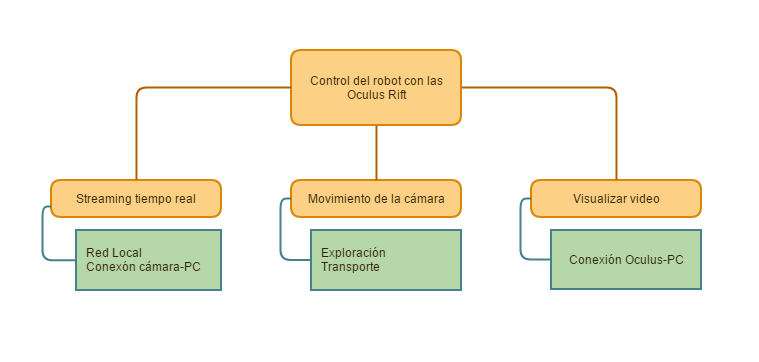
\includegraphics[width=7.00in]{images/objetivos.png}}
	}
	\caption{Resumen de los objetivos del proyecto}
\end{figure}

\newpage
\section{Estructura del documento}


El objetivo de este documento es explicar el trabajo realizado y los resultados obtenidos.

En el siguiente capítulo se explica el estado del arte, hablando brevemente de la realidad virtual y de algunos proyectos previos que utilizaban esta tecnología. Como se verá más adelante el capítulo se centra especialmente en proyectos relativos a salud y robótica.

Luego se verá el análisis, diseño y desarrollo del proyecto.

En el análisis se presentan los requisitos que debe cumplir nuestro sistema. Posteriormente se hace un estudio de diseño de los componentes del trabajo (robot, conexiones entre dispositivos...) y por último se explicará como se ha desarrollado el proyecto.

Los resultados y las pruebas realizadas para ver si el proyecto cumplía con el objetivo se verán en el capítulo "Pruebas y resultados" de este documento.

Para finalizar expondremos brevemente las conclusiones y el trabajo futuro que se puede realiza en base a este proyecto.

\chapter{Estado del arte}

\section{Introducción}
En este capítulo se contará brevemente la historia de la realidad virtual.
También se presentarán diferentes proyectos que ha utilizado realidad virtual y robótica y cuales fueron sus resultados.

De esta forma se dará una fotografía general del estado y las aplicaciones actuales de ambas tecnologías, dando especial importancia a aquellos proyectos con un enfoque similar al de nuestro trabajo.

\subsection{Historia}
La realidad virtual comenzó siendo ciencia ficción y poco a poco está ganando terreno en la vida cotidiana, ya sea en el mundo de los videojuegos, la medicina o la aviación, entre otros campos.

A pesar de ser una tecnología de la que se ha empezado a hablar hace relativamente poco, los primeros proyectos que utilizaban realidad virtual datan de los años 60.

Uno de los  acontecimientos más significativos del inicio de la realidad virtual es la creación de \textbf{“The Sword of Damocles”} , un casco de realidad virtual (HMD- head-mounted display)  creado por Ivan Sutherland en 1968 \cite{Sutherland}.

The Sword of Damocles permitía ver las imágenes tridimensionales generadas por el
ordenador superpuestas ópticamente, a través de un prisma, al entorno real que rodeaba al usuario.

 El sistema estaba montado sobre un brazo mecánico suspendido del techo que también servía para detectar, mediante el uso de sensores, la posición y la orientación de la cabeza del usuario. De este modo, cuando el usuario se movía, los objetos creados por el ordenador daban la impresión de encontrarse en una posición estable dentro del entorno real.

Es lógico preguntarse cómo ha tardado tanto en llegar al mercado la realidad virtual si ya en 1968 consiguieron sacar adelante este proyecto.

La respuesta es que \textbf{la tecnología de los años 60 aún no estaba preparada} para desarrollar herramientas de realidad virtual.

Para conseguir capturar la posición y el movimiento de la cabeza del usuario, se requería un brazo de \textbf{grandes dimensiones}.
Además la realidad virtual necesita una \textbf{capacidad de cómputo muy potente}. Problemas tales como "hidden line" solo podía ser resueltos con un ordenador que tenía la NASA en Houston, como especifica Sutherland en su trabajo \textit{A head-mounted three dimensional display} \cite{Sutherland}. 

\begin{figure}[h]
	\centerline{
		\mbox{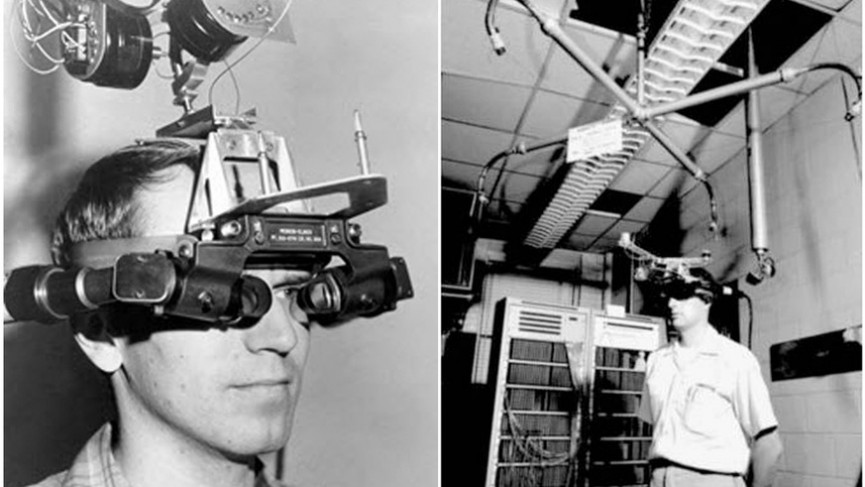
\includegraphics[width=.80\textwidth]{images/SwordOfDamocles.jpg}}
	}
	\caption{Sword of Damocles. Imagen obtenida de \textit{A head-mounted three dimensional display} \cite{Sutherland}}
	
\end{figure}


Al mismo tiempo Thomas A. Furness III empezó a introducir herramientas de \textbf{realidad virtual en entrenamientos de vuelo} \cite{kocian1977visually}, con el objetivo de que estos fueran mucho más seguros para los pilotos.
A pesar de que fue una gran aportación en este campo, la escasez de recursos y capacidad de cómputo también retrasaron mucho el desarrollo de estas herramientas.
 
Hoy en día tenemos la capacidad necesaria para desarrollar estas herramientas por lo que se siguen utilizando y mejorando ya que, no solo es más segura, sino que además es más barata.

Durante las últimas décadas del s.XX, se hicieron algunos proyectos de realidad virtual , pero no tuvieron mucho éxito debido a su alto coste.

Con el desarrollo exponencial que ha vivido la tecnología las últimas décadas, la realidad virtual ha ido haciéndose un hueco en la industria tecnológica.
El empujón definitivo vino con la creación de las \textbf{Oculus Rift}, en el año 2010.

\textbf{Palmer Luckey} es el fundador de Oculus VR (una compañía de realidad virtual) y el diseñador de la primera versión de las Oculus Rift.

Oculus Rift es un casco de realidad virtual (también nos podemos referir a ellas como gafas de realidad virtual) mucho más manejable que "The Sword of Damocles" , con muchas más calidad y con un coste asequible.
Uno de los grandes logros de Luckey con las Oculus Rift es que consiguió un ángulo de visión de 90º, algo nunca visto hasta el momento.

Tras el lanzamiento de las Oculus Rift, el mercado comenzó a interesarse por proyectos relacionados con la realidad virtual y a financiarlos.
Gracias a esto la tecnología ha podido desarrollarse y hoy podemos disfrutar de una realidad virtual con mucha más calidad y \textbf{sensación casi total de inmersión} en entornos virtuales.

La cara más visible de la realidad virtual es el uso que se le da en los videojuegos pero no es su única aplicación.

A continuación se presentarán diferentes proyectos donde se utiliza la realidad virtual en el campo de la salud, sobretodo aplicada a rehabilitaciones. Esto es muy interesante para este trabajo ya que muestra cómo usuarios con alguna dificultad motora responde bien a entornos virtuales.

También se hablará de cómo se están integrando actualmente  las dos tecnologías que utilizaremos en este trabajo: la robótica y la realidad virtual.


\section{Realidad virtual y salud}
\label{sec:VR y salud}

El uso de realidad virtual está siendo muy útil en medicina, ya que permite crear diferentes entornos y estudiar cómo responde y  es capaz de interactuar el paciente en distintas situaciones de forma bastante realista.

Un ejemplo de esto es la evaluación del deterioro cognitivo en personas que sufren esclerosis múltiple. Para dicha evaluación se requiere una gran cantidad de datos sobre la velocidad de procesamiento de la información, atención, etc.Esto se conseguía haciendo múltiples test que no siempre eran fieles a la realidad.

Ahora con la Realidad Virtual se consiguen crear entornos en los que el usuario tiene tal sensación de inmersión, que su comportamiento es muy similar al que tendría en el entorno real. Esto permite hacer un estudio mucho más amplio y realista de los estímulos del paciente y obtener resultados más completos.\cite{LamargueHamel201594}


También se está estudiando el uso de programas de rehabilitación para que los pacientes no necesiten trasladarse hasta el hospital.

Uno de los estudios se hizo a personas con hemiparesia, con un software que mostraba por pantalla el movimiento de los pies y les mandaba ejercicios para mejorar su capacidad motora. Los resultados de este estudio mostraron que la herramienta de realidad virtual era efectiva para la rehabilitación y muy útil para los pacientes con dificultades para trasladarse hasta el hospital[ref]





\section{Robótica y realidad virtual.} 
\label{sec:robotica y VR}
La unión de robótica y realidad virtual es algo que se lleva haciendo desde hace bastante tiempo.

En el campo de la salud una de las aplicaciones son entrenamientos de cirug´ia. La realidad virtual permite crear un entorno semejante al quir´ofano. El estudiante hace uso de herramientas que simulan los utensilios quir´urgicos y puede hacer una "operaci´on virtual" sin riesgo para ning´un paciente y sin necesidad de gastar recursos o un equipo quir´urgico de apoyo . [ref]

En educación hay varios programas de realidad virtual que hacen el aprendizaje más sencillo y completo a los estudiantes. Un ejemplo de esto es la visualización de brazos robóticos para diseñar correctamente el movimiento.
Es relativamente complejo traducir cada movimiento de las articulaciones del brazo robótico en la posición finla de éste. Si estas pruebas se hicieran directamente sobre el robot, sería muy sencillo romperlo. Con los programas de realidad virtual se simulan todos los movimientos sin peligro de malgastar recursos. [ref]

Otra aplicación es el control remoto de robots, tanto con software que crea una interfaz virtual para que el usuario obtenga de forma clara toda la información del robot (batería, almacenamiento de datos, posición...) [ref NASA xD], como interfaces BCIs.


\chapter{Análisis, diseño y desarrollo}
\label{chap:sistemadesarrollado}
Este capítulo explica las fases que se han llevado a cabo para desarrollar el proyecto.

La primera fase es la de análisis. Se estudia el objetivo y los requisitos que debe cumplir. De esta forma el trabajo queda dividido en pequeñas tareas y facilita su implementación.

La sección de diseño explica las herramientas que se han utilizado para implementar cada parte y cómo funcionan.

Por último se explica de forma más detallada cómo se ha desarrollado cada parte del problema, qué dificultades han ido apareciendo y cómo se han solucionado. También explica cómo se ha realizado la integración para conseguir el proyecto final.

\section{Análisis}
En el capítulo de \textit{Objetivos} se explica que la meta final del proyecto es conseguir que el usuario pueda controlar una cámara con el movimiento de cabeza y ver todo lo que la cámara vea.

La forma más eficiente de hacer que la cámara sea móvil es construir un robot con ruedas que lleve la cámara integrada. 

De esta forma cuando el usuario mueva la cabeza, se le enviarán las instrucciones necesarias al robot para que se mueva. A su vez el robot le estará mandando video a tiempo real al usuario, que lo verá a través de las Oculus Rift.

DIBUJO CHULI DE TODO JUNTO

El proyecto por lo tanto se divide en 3 problemas:
\begin{enumerate}
	\item Construcción del robot $\rightarrow$ para ello necesitaremos una placa base, una cámara y la estructura que le permita desplazarse.
	\item Streaming $\rightarrow$ Debemos conseguir transmitir a tiempo real todo lo que ve el robot a la Oculus
	\item Control del robot$\rightarrow$ Queremos que el robot sea una extensión de los sentidos del usuario, por lo que debemos idear movimientos intuitivos para que el usuario mande comandos de movimiento al robot.
\end{enumerate}

Vamos a desarrollar cada uno de ellos, identificando qué funcionalidades básicas debe cumplir.

\subsection{Requisitos Funcionales}

\subsubsection{Construcción del Robot}


El robot debe ser un dispositivo fácil de controlar , que a su vez actúe como una extensión de los ojos del usuario, dándole a éste la sensación de inmersión en un espacio real o virtual.

Por tanto los requisitos que debe cumplir el robot son los siguientes:


\begin{itemize}
	\item \textbf{RF-CR1}
	
	Permitir grabar video y transmitirlo a tiempo real.
	
	
	\item\textbf{RF-CR2} 
	
	Ser capaz de desplazarse en todas las direcciones
	
	
	\item\textbf{RF-CR3}
	
	Tener la capacidad de recibir comandos de control a través de una red inalámbica
	
	
	\item\textbf{RF-CR4} 
	
	Ser capaz de que la cámara apunte en la misma dirección que la cabeza del usuario
\end{itemize}

DIBUJO AMPLIADO ROBOT

\subsubsection{Streaming}

Se quiere conseguir la máxima sensación de inmersión para la persona que controla el robot.

Para ello los requisitos principales que debe cumplir son:

\begin{itemize}
	\item\textbf{RF-S1}
	
	La transmisión de video debe ser  a tiempo real, con la mínima latencia posible.
	
	\item\textbf{RF-S2}
	
	El usuario verá el video con  las Oculus Rift, por lo que la imagen debe estar desdoblada (formato SBS, que se eplicará en la sección de desarrollo).
	
	\item\textbf{RF-S3}
	
	La transmisión debe ser inalámbrica ya que queremos que el robot tenga total libretad de movimiento, siendo éste independiente del ordenador.
	
	
	Dado que la placa que utilizamos en el el robot es la Raspberry Pi 3 tenemos dos opciones para la transmisión inalámbrica: Bluetooth o red Wifi.
	
\end{itemize}



\subsubsection{Control del Robot}

Como hemos dicho anteriormente, el robot pretende ser una extensión de los ojos de usuario, por lo que es lógico que se controle con el movimiento de cabeza de la persona que esté recibiendo el video.

Dentro del control del robot vamos a diferenciar entre control del movimiento del robot y control de la dirección de la cámara:

\begin{itemize}
	\item Movimiento del robot :
	
	\textbf{RF-CTRL1}
	
	Debemos diseñar un sistema intuitivo para mover el robot en todas las direcciones con movimientos de la cabeza.
	\item  Movimiento de la cámara:
	
	\textbf{RF-CTRL2}
	
	La cámara debe estar apuntando siempre en la misma dirección que la cabeza.
	
	Si el usuario mueve la cabeza hacia la derecha o hacia la izquierda, el robot se moverá en esa dirección, por lo que no hay que preocuparse por la cámara.
	
	Para controlar los movimientos verticales vamos a incorporar un servo unido a la cámara, de forma que ésta se mueva en función de la posición de la Oculus. 
\end{itemize}


\subsection{Requisitos no funcionales}

\begin{itemize}
	\item \textbf{RNF1 - Usabilidad}
	
	
	El sistema para controlar el movimiento del robot y de la cámara debe ser intuitivo, sin requerir movimientos de cabeza inusuales por parte del usuario.
	
	
	
	\item \textbf{RNF2 - Documentación}
	
	El usuario debe disponer de un manual de uso sencillo para poder utilizar correctamente el sistema .
\end{itemize}

\newpage
\section{Diseño}

Tras analizar las diferentes funcionalidades del trabajo vamos a ver cómo está diseñado cada componente.

Los principales dispositivos que componen el proyecto son 
\begin{itemize}
	\item Robot
	\item Router
	\item Oculus Rift
\end{itemize}

También se tratará el \textbf{diseño de conexiones} entre los 3 componentes.

\subsection{Diseño del robot}

El robot que se utiliza en este proyecto está basado en un diseño anterior hecho por (Nombre del alumno que diseñó en robot)

Consta de:
\begin{itemize}
	\item Una placa base $\rightarrow$ Raspberry Pi 3
	\item Dos ruedas conectadas con dos servos que permiten al robot desplazarse.
	\item Una cámara Logitech, conectada a la placa por USB
	\item Un servo conectado a la cámara 
\end{itemize}


FOTO ROBOT

\subsubsection{Raspberry Pi 3 model B}

La Raspberry Pi 3 model B es un ordenador de placa reducida que lleva un sistema operativo Linux.

Su procesador es un ARM Cortex A53 de cuatro núcleos a 1.2GHz de 64 bits.

Tiene 1 GB de memoria RAM , 4 puerto USB, 40 pins GPIO, puerto HDMI , Ethernet y entrada para MicroSD.

Además tiene Wifi 802.11n integrado y bluetooth 4.1.


\begin{figure}[h]
	\centerline{
		\mbox{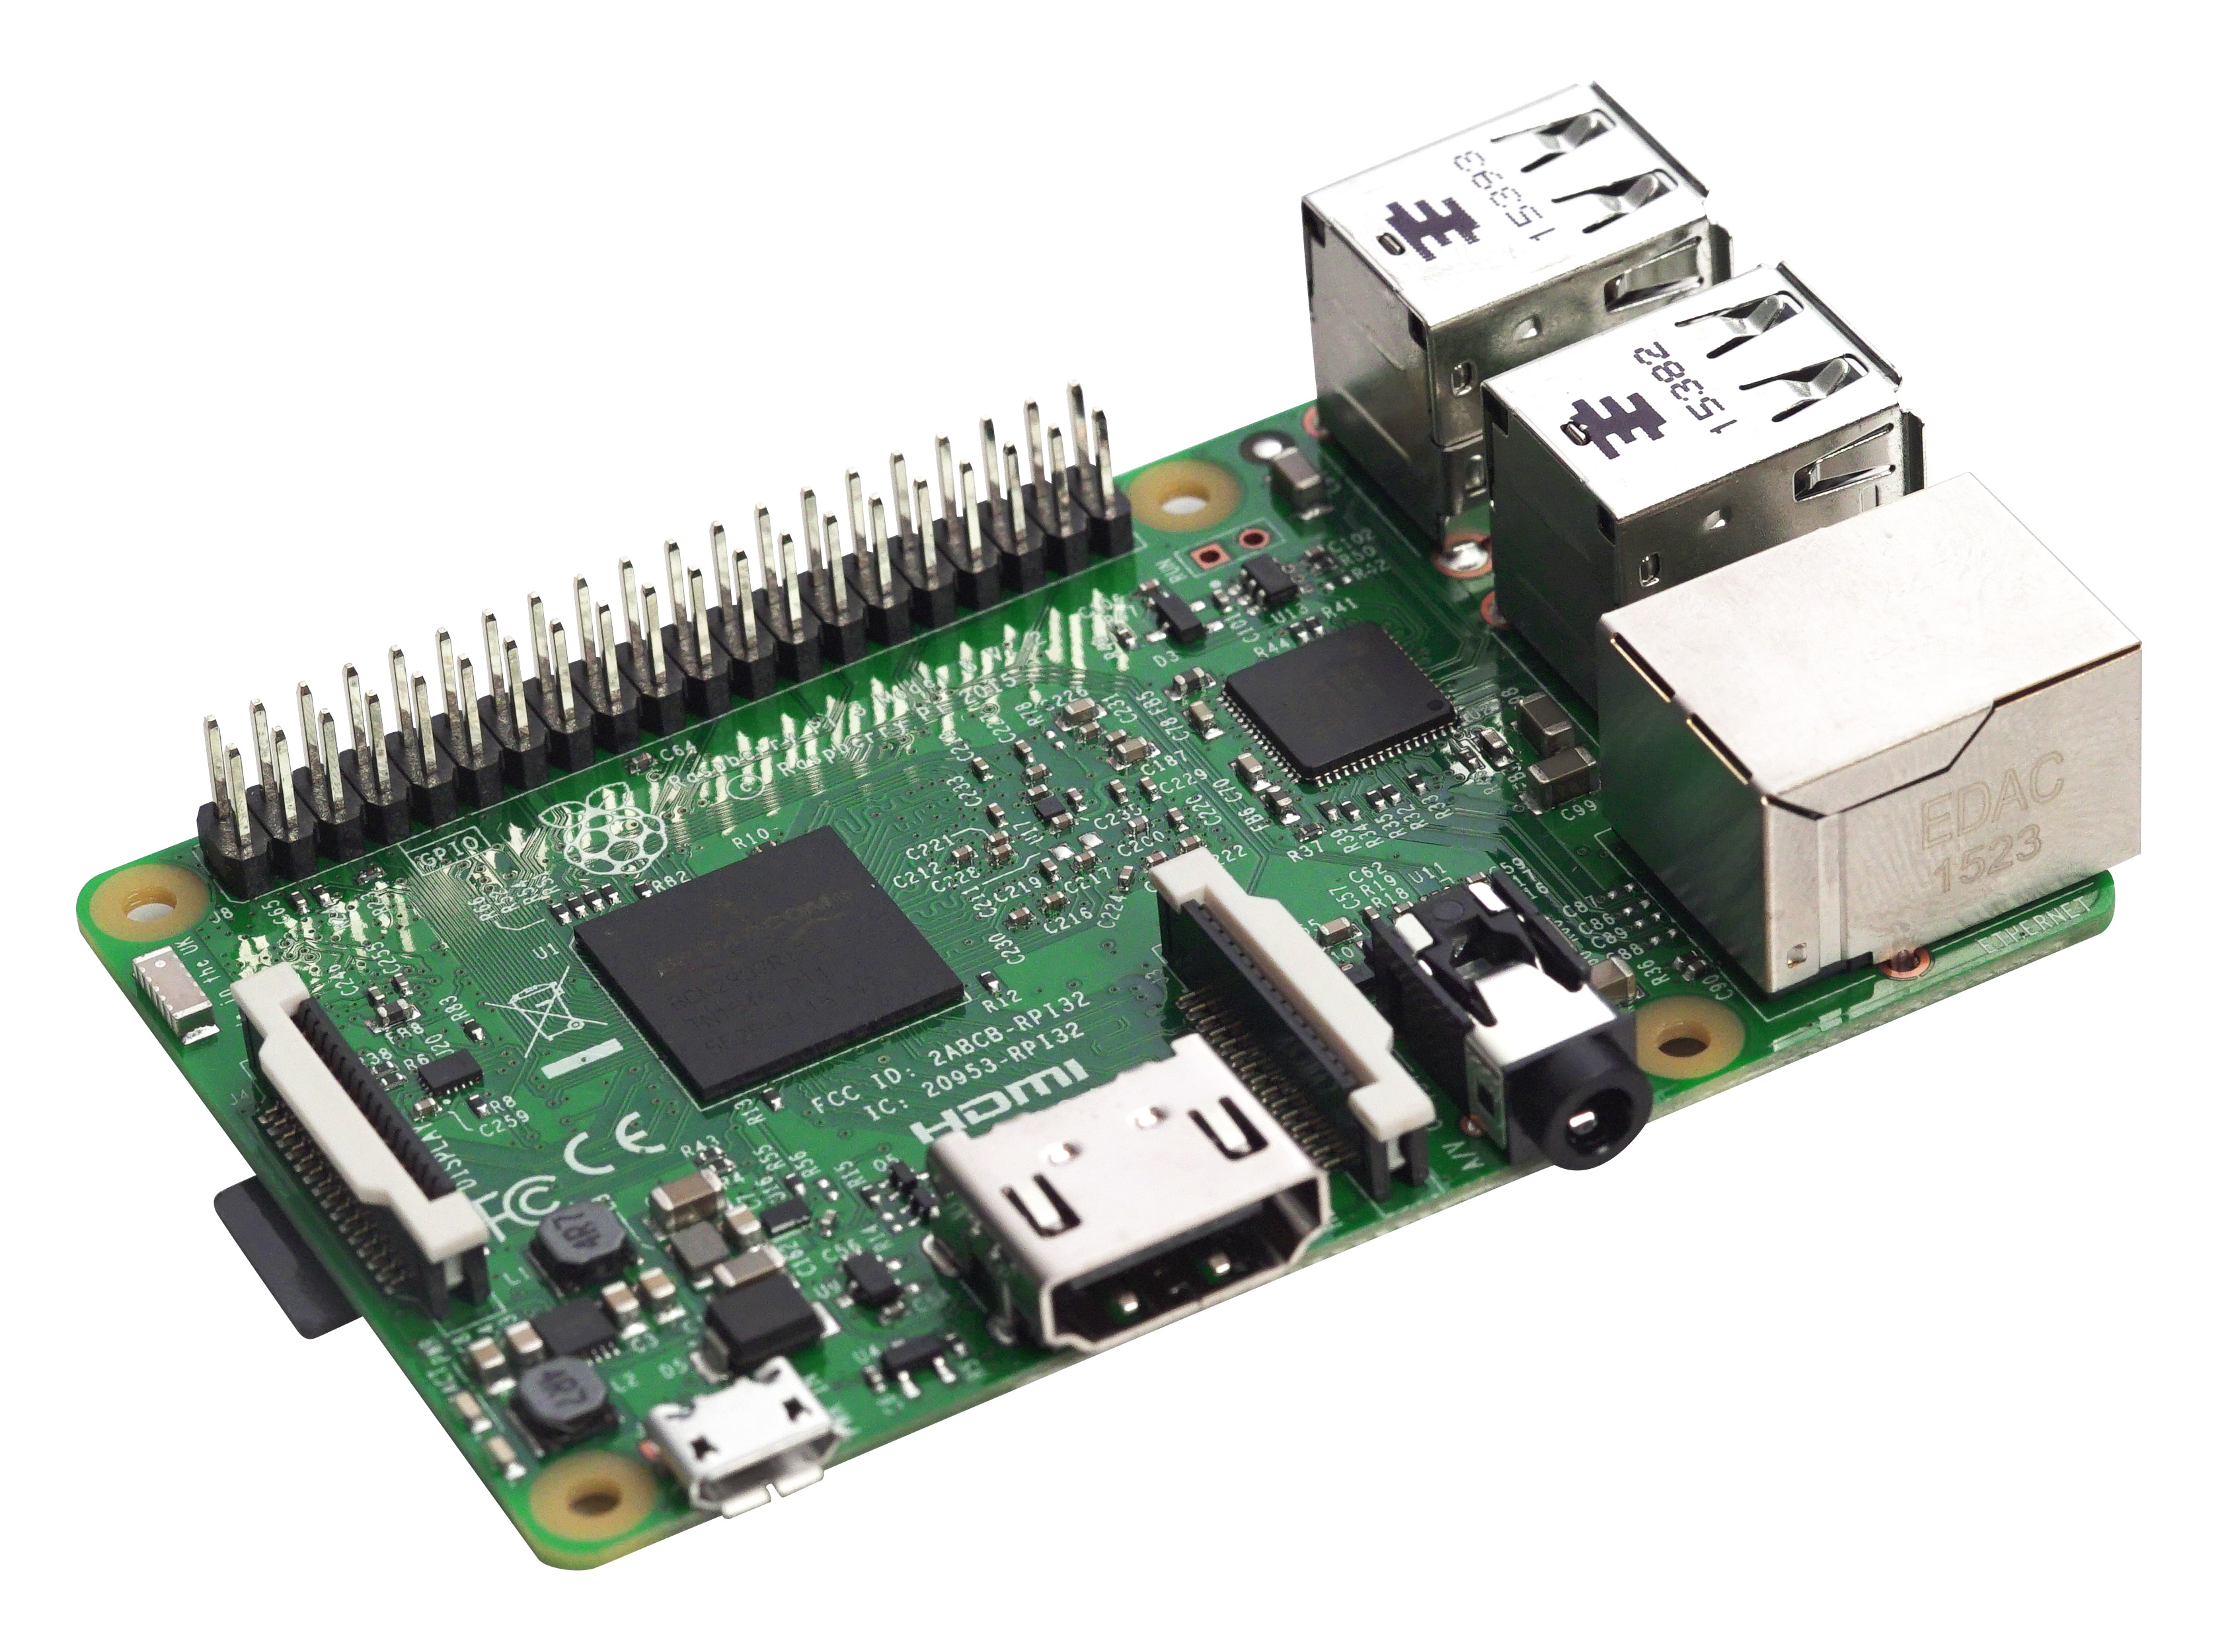
\includegraphics[width=.80\textwidth]{images/raspi3.jpg}}
	}
	\caption{Raspberry Pi 3 model B}
	
\end{figure}

\subsubsection{Servo motores}
Para el movimiento del robot y de la cámara utilizamos servo motores


Un servo motor es un motor eléctrico que se puede controlar su velocidad y su posición (dentro del rango de posición permitido).

Los servos constan de:
\begin{itemize}
	\item Un motor de corriente continua
	\item Una caja reductora
	\item Un circuito de control
\end{itemize}

El sistema que utilizamos para controlar la velocidad y la posición de los servos es la modulación por anchura de pulso (PWM).

\paragraph{PWM}

Este sistema consiste en generar una onda cuadrada en la que se varía el tiempo que el pulso está a nivel alto, manteniendo el mismo período (normalmente), con el objetivo de modificar la posición del servo según se desee.

\begin{figure}[h]
	\centerline{
		\mbox{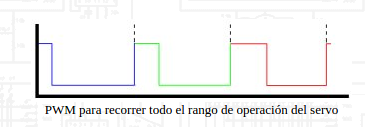
\includegraphics[width=.80\textwidth]{images/ondaServo.png}}
	}
	
\end{figure}



Para que un servo se mantenga en la misma posición durante un cierto tiempo, es necesario enviarle continuamente el pulso correspondiente.


La otra función del PWM hemos diche que era el control de velocidad.

Esto lo hace alimentando el motor con una señal de pulsos con la frecuencia suficiente para que el motor no note las variaciones y haga un giro constante, ya que variando el porcentaje de tiempo de la señal rectangular en alta, y en baja, variamos la potencia que le entregamos al motor, con lo que controlamos la velocidad de giro con mucha precisión.

En el robot utilizamos 3 servomotores.
Dos de ellos se utilizan para el movimiento de las ruedas y el tercero moverá la cámara permitiendo al usuario mirar hacia arriba y hacia abajo.

Los tres servos están controlados por el movimiento de la cabeza del usuario, que obtenemos gracias a las Oculus Rift.

\subsubsection{Cámara}

La cámara utilizada es una webcam USB. El proyecto también se podría haber hecho con una RaspiCam.

A continuación se muestra un esquema de la conexión entre los componentes que acabamos de explicar.


\begin{figure}[h]
	\centerline{
		\mbox{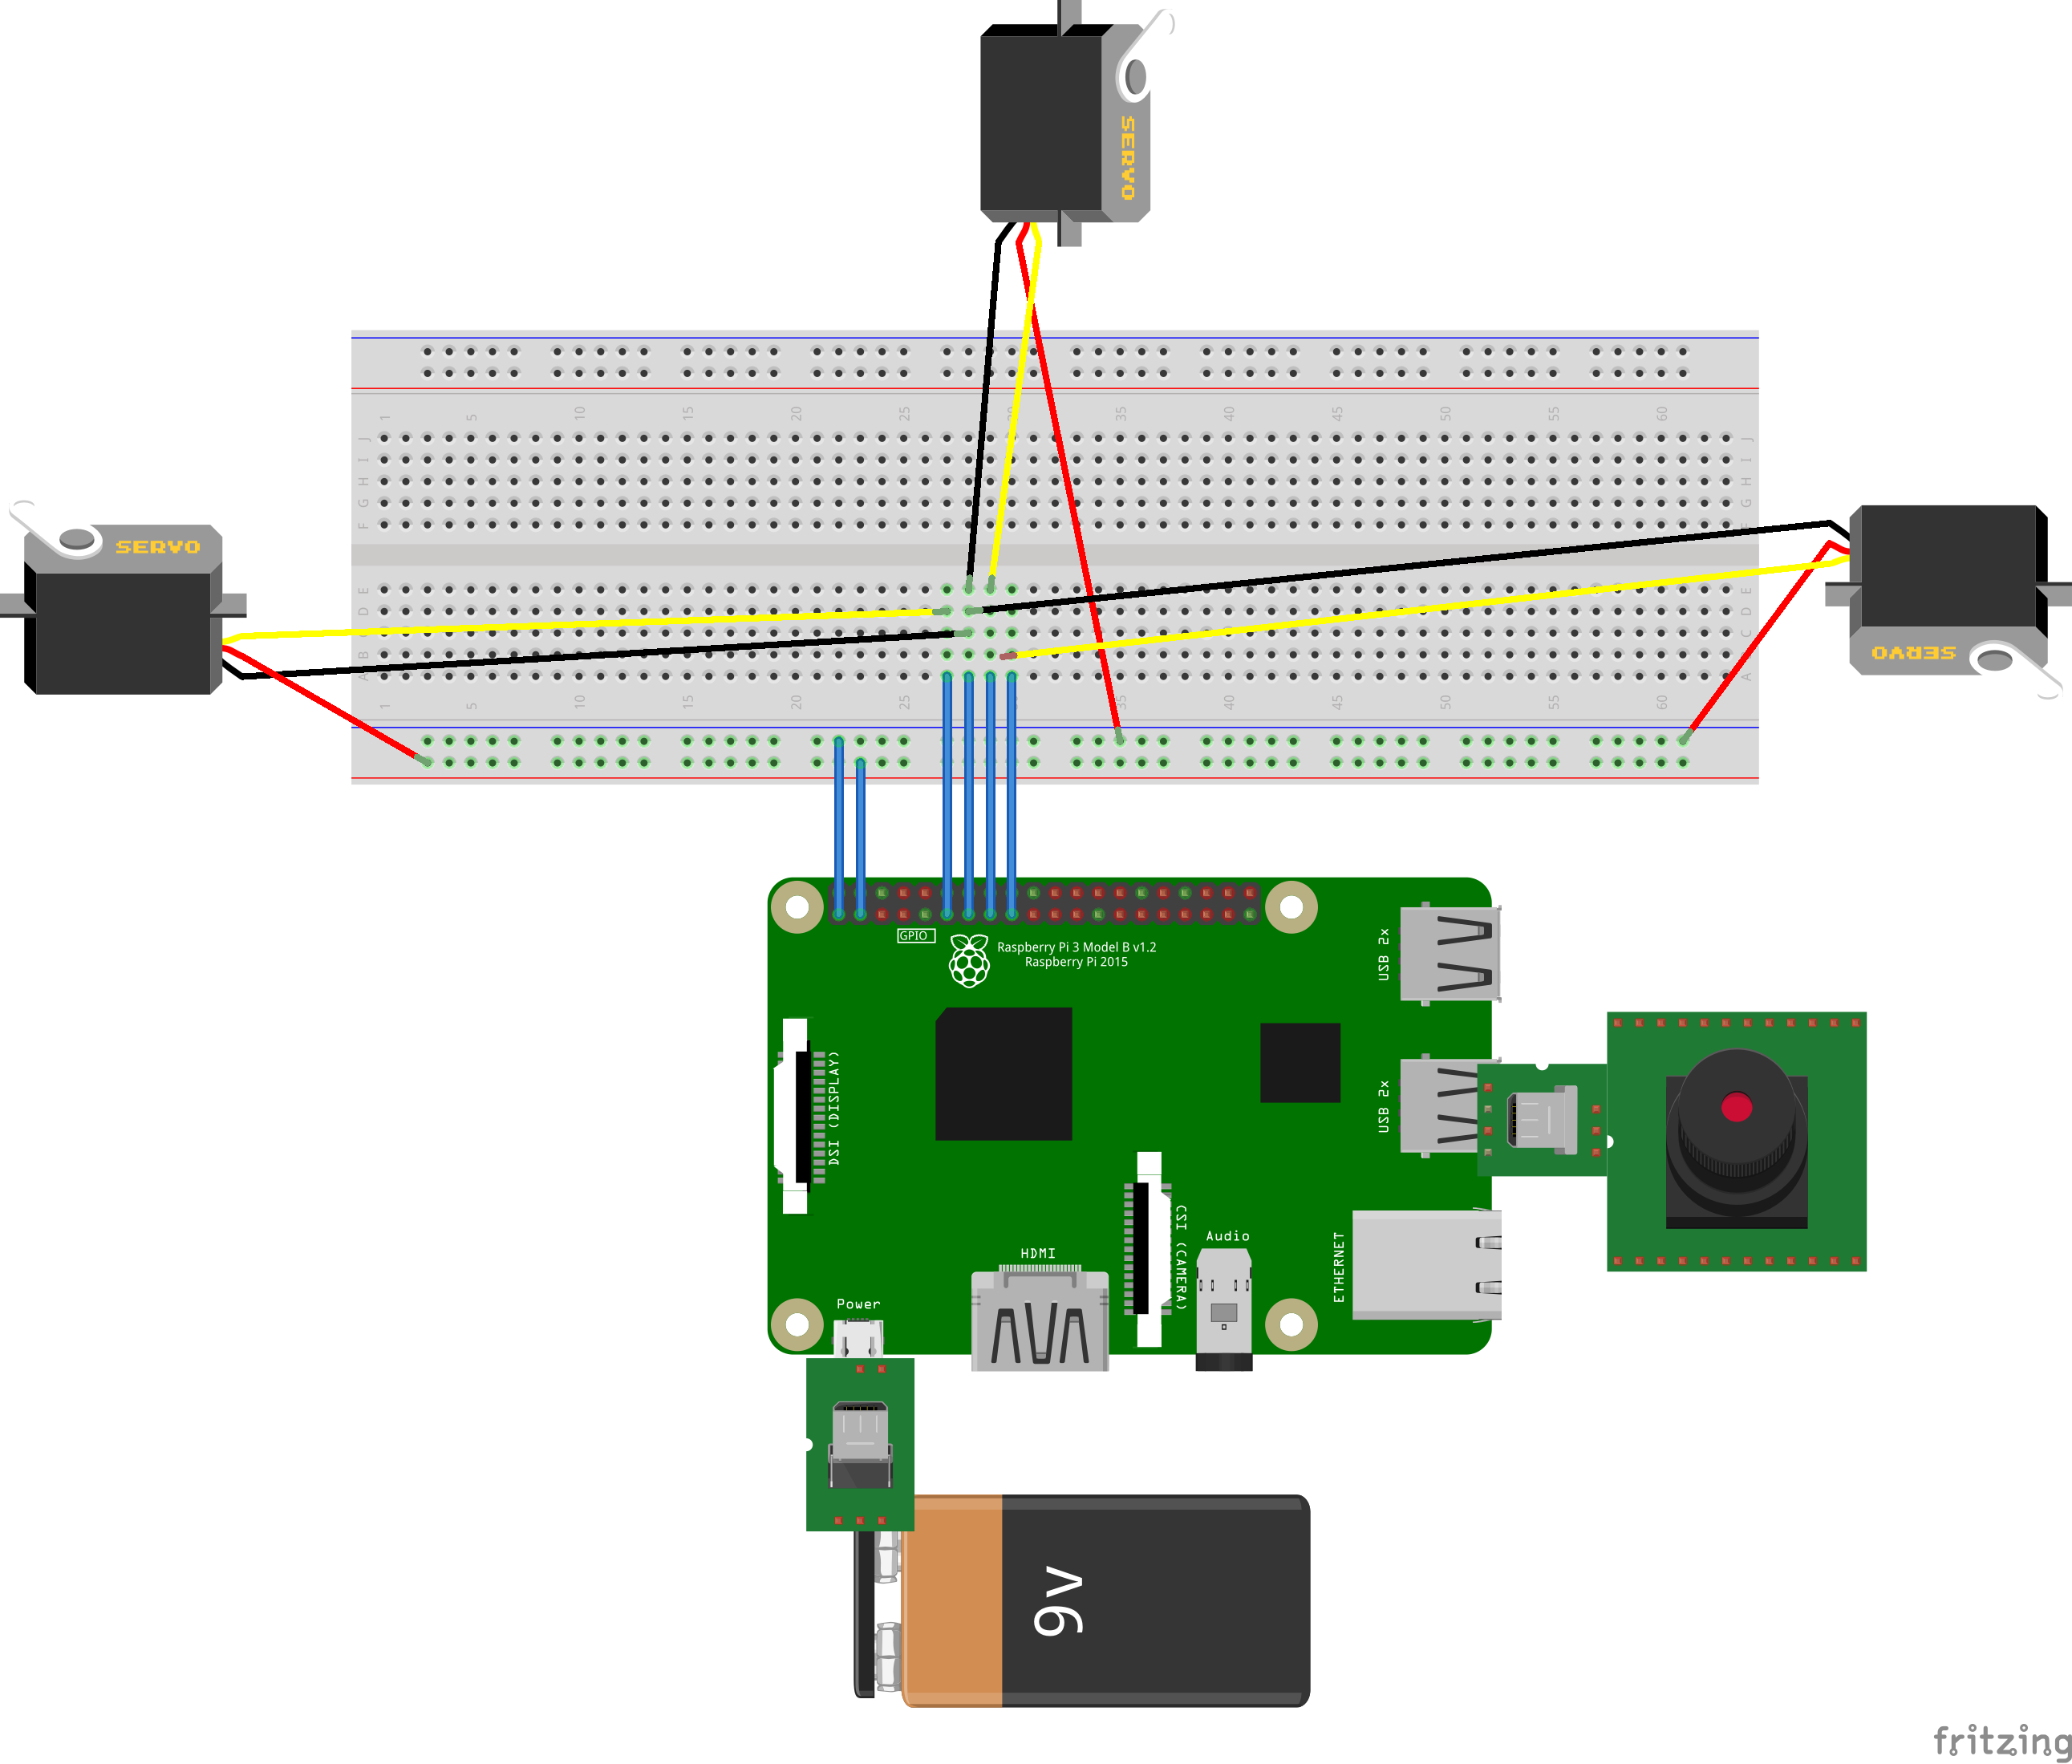
\includegraphics[width=.95\textwidth]{images/EsquemaServos.png}}
	}
	\caption{Esquema conexiones servos , cámara, Raspberry Pi 3}
\end{figure}


\subsection{Router}
Para la comunicación entre el robot y el ordenador se necesita una red local,  para este trabajo la hemos creado haciendo uso de un router inalámbrico Xavi7968.

El router crea una red Wifi con el nombre de WifiRaspi3 y sin acceso a internet.

Para una mayor facilidad de conexión se ha configurado la tabla DHCP del router para asignar siempre la misma IP a la Raspberry y al equipo que utilizamos para conectarnos.

\begin{figure}[h]
	\centerline{
		\mbox{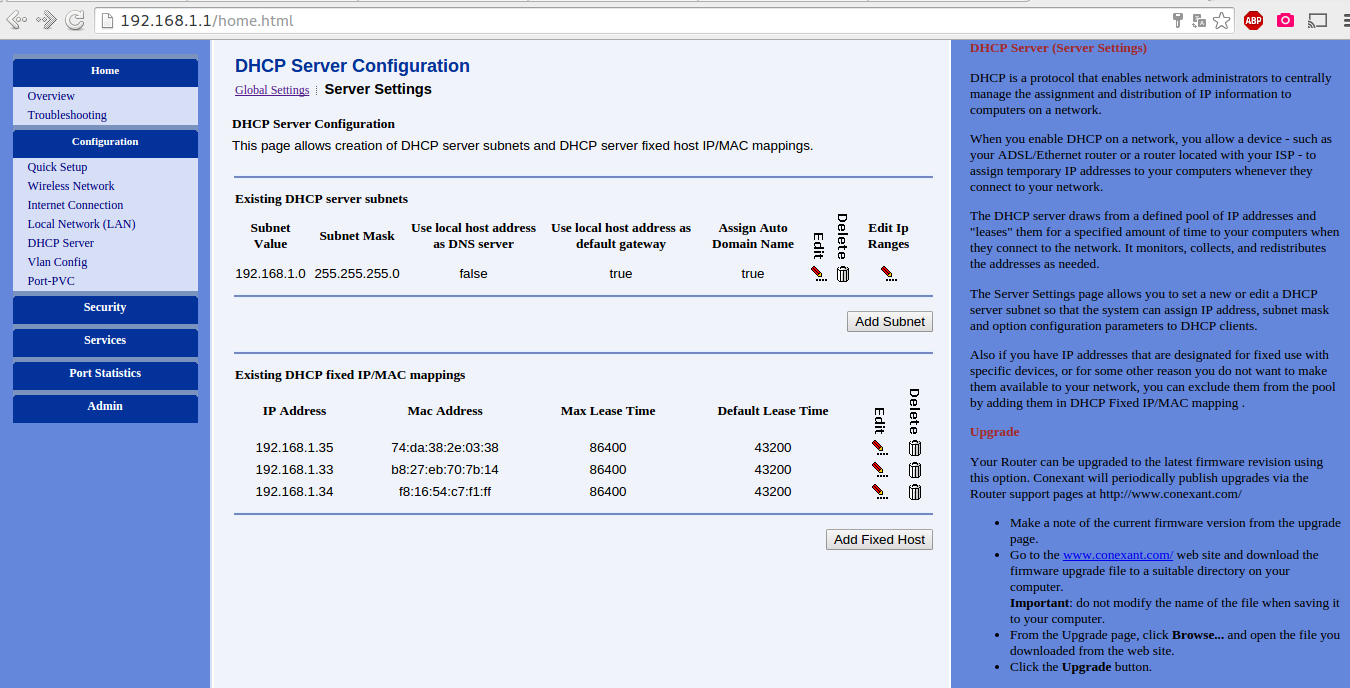
\includegraphics[width=.95\textwidth]{images/TablaDHCP2.png}}
	}
	\caption{Tabla DHCP del router con las parejas MAC-IP fijas}
\end{figure}

La Raspberry Pi 3 está configurada para conectarse automáticamente al router. Para ello se ha modificado el archivo \texttt{/etc/wpa\_supplicant/wpa\_supplicant.conf} donde se especifica el nombre y la clave de la red local.

\begin{figure}[h]
	\centerline{
		\mbox{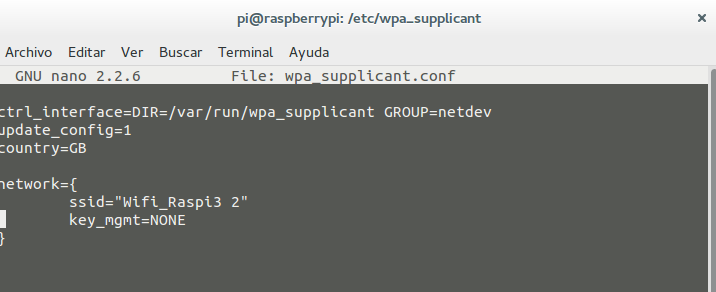
\includegraphics[width=.95\textwidth]{images/confRaspiWifi.png}}
	}
	\caption{Archivo de configuración de red Raspberry Pi 3}
\end{figure}
 

\subsection{Oculus Rift}

Las Oculus Rift son unas gafas de Realidad Virtual [parrafo definiendo las Oculus]

De las gafas nos interesan especialmente:
\begin{itemize}
	\item Detección de la orientación de las Oculus
	\item Recepción de video
\end{itemize}

\subsubsection{Detección de la orientación}



Las Oculus Rift tienen integradas un giroscopio, un acelerómetro y un magnetómetro que manda constantemente información al ordenador, de forma que éste sabe en todo momento la orientación de las gafas.

La técnoca para interpretar la señal de estos sensores se llama \textbf{fusión de sensores}

A continuación se explica en qué consiste esta técnica.

\paragraph{Fusión de Sensores }

Como ya hemos mencionado, en las Oculus tenemos un giroscopio, un acelerómetro y un magnetómetro.

Los dos primeros dan información acerca de la orientación respecto a los ejes X y Z, mientras que el magnetómetro mide la orientación respect al eje Y.

Vamos a ver cómo funciona cada uno.

El \textbf{giroscopio} de las Oculus mide el cambio de orientación de la cabeza a una velocidad de 1KHz.

Una forma simplificada de calcular la orientación actual es:

$$\text{Orientación actual } = \text{ Orientación anterior } + \text{ Diferencia horaria } \cdot \text{ Velocidad observada (giroscopio).}$$

El problema está en que la cabeza puede rotar alrededor de tres ejes.

\begin{figure}[h]
	\centerline{
		\mbox{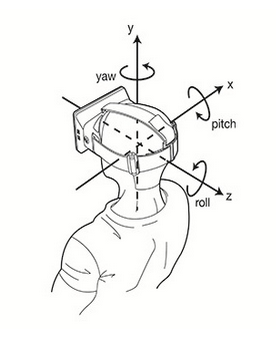
\includegraphics[width=3.00in]{images/headtracking.png}}
	}
	\caption{Ejes de giro}
\end{figure}

Vamos a suponer que solo rotase alrededor del eje Y y que el sensor captase una velocidad angular $w$ por segundo.

Si tuviéramos 1000 sensores la fórmula de la orientación sería:

$$\text{Orientación actual } = \text{ Orientación anterior } + 0,001 \cdot w$$

Pero en el caso de las Oculus, al estar midiendo un objeto que se mueve en 3 ejes, el giroscopio da la velocidad angular respecto de los tres ejes, devolviendo un vector 3D ($w_1,w_2,w_3$)

Al basar nuestro cálculo en el cálculo anterior, el error irá creciendo con el tiempo.

Vamos a llamar \textit{tilt error} al error en la medición de los ángulos sobre los ejes XZ. El error sobre el eje Y se llamará \textit{yaw error}.

El \textit{tilt error} se corresponde con nuestra sensación de lo que "está arriba", percepción que se basa en la gravedad.

La gravedad se expresa con un vector de aceleración , por lo que utilizamos un \textbf{acelerómetro} para medirla.

Nos encontramos con el inconveniente de que el acelerómetro no solo mide la gravedad. Para asegurarnos de que el momento en el que tomamos los datos de referencia solo estamos midiendo la gravedad, esperamos a que se den 2 condiciones:
\begin{enumerate}
	\item El acelerómetro nos devuelve una medida cercana a 9,8
	\item El giroscopio nos devuelve una velocidad angular muy lenta (es decir, no estamos girando).
\end{enumerate}

En este momento sabemos que nos encontramos en una posición vertical y podemos corregir el error.

\textbf{Cómo corregimos el error:}
Supongamos que se dan las dos condiciones previas, y la posición que nuestro cálculo de orientación nos devuelve un vector $\vec{a}$, tal y como vemos en el dibujo.

Tenemos el ángulo $\theta$ entre el eje Y y el vector $\vec{a}$ pero ¿cómo calculamos el eje de rotación para rotar $\vec{a}$ y corregir el error?

Dicho vector debe ser perpendicular a $\vec{a}$ y al eje Y, y apoyarse en el plano XZ.

Para encontrar el vector basta con hacer la proyección de $\vec{a}$ en el plano XZ, obteniendo así ($a_x, 0 , a_z$). Haciendo un vector perpendicular a éste obtenemos ($-a_z, 0 , a_x$). Y ya tenemos el eje de rotación que necesitabamos para corregir el error.

\begin{figure}[h]
	\centerline{
		\mbox{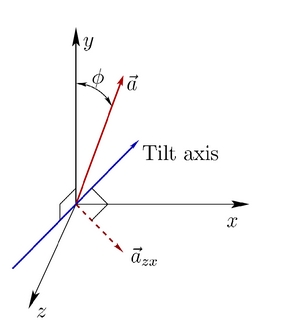
\includegraphics[width=3.00in]{images/ejestracking.png}}
	}
	\caption{Corrección del tilt error}
\end{figure}


\newpage
\textbf{Error sobre el eje Y (yaw error)}

Este error se basa en nuestra percepción de dónde está el norte.

Para esto utilizamos el magnetómetro.

El procesamiento de la señal del magnetómetro y la corrección del error es similar al tratamiento de la señal del giroscopio.

\subsection{Diseño de conexiones}

La arquitectura del proyecto es muy sencilla, como podemos observar en la siguiente imagen:

\begin{figure}[h]
	\centerline{
		\mbox{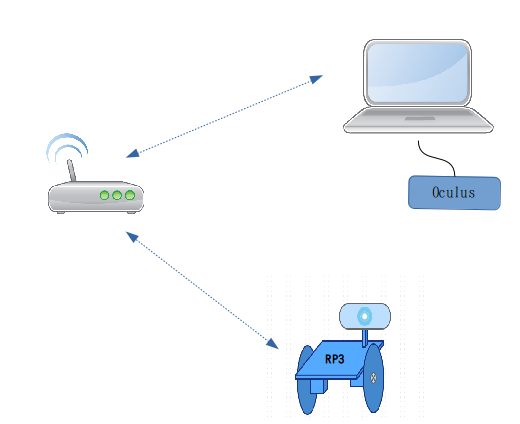
\includegraphics[width=.80\textwidth]{images/EsquemaConexiones.png}}
	}
	\caption{Esquema conexiones}
\end{figure}


Como podemos ver en el esquema, las Oculus Rift están conectadas al ordenador, el ordenador y la Raspberry se mandan información a través de un router que crea una red local.

La raspberry recibe en streaming de la cámara y lo va mandando a una IP disponible dentro de la red local, la (192.168.1.35). A su vez el ordenador accede a esa IP, recoge el streaming utiliza VLC para dividir la imagen (SBS) y reproducir el video y con la herramienta Virtual Desktop podemos ver el video desde las Oculus.

Por otra parte las Oculus tienen integrado un giroscopio , un acelerómetro y un magnetómetro.

Combinando la información de estos sensores a través de un proceso conocido como fusión de sensores se determina la orientación de la cabeza del usuario en el mundo real , y se sincroniza con la perspectiva virtual del usuario en tiempo real. 

Se ha implementado un programa en phyton que recoge esa información y la traduce en comandos sencillos para mandarselos a la Raspberry. Para obtener esa información hacemos uso de la librería de las Oculus (ovr).

La Raspberry lee los comandos del ordenador y mueve los servos según lo recibido, de esta forma controlamos el movimiento del robot y de a cámara.

\newpage
\section{Desarrollo e implementación}
En esta sección se explicará cómo hemos desarrollado las distintas funcionalidades del proyecto.
Para ello vamos a diferenciar entre:

\begin{itemize}
	\item Construcción del Robot
	\item Streaming 
	\item Control del Robot
\end{itemize}

Para conseguir \textbf{transmitir a las Oculus el video en tiempo real} es necesario que:
\begin{enumerate}
	\item La Raspberry recoja el video de la cámara y lo transmita al ordenador.
	
	\item El ordenador recoja el video, lo transforme a formato SBS y lo envíe a las Oculus Rift. 
	
\end{enumerate}





Para el \textbf{control del robot} se deberán implementar las siguientes tareas:

\begin{enumerate}
	\item Leer la señal de los sensores de las Oculus Rift (giroscopio, acelerómetro y magnetómetro) para saber la orientación de la cabeza del usuario.
	
	\item Transmitir la información obtenida al robot.
	
	\item Traducir dicha información en comandos para mover los servo motores.
\end{enumerate} 
\subsection{Construcción del Robot}
Como se ha dicho en la sección de diseño, el robot está construido basándose en el diseño de un robot de un trabajo anterior.

Para este proyecto se han añadido alguno componentes:

\begin{itemize}
	\item Soporte de la cámara
	\item Batería portátil
\end{itemize}

\subsubsection{Soporte de la cámara}

Para integrar la cámara en el robot han sido necesarias dos piezas:

\begin{itemize}
	\item Soporte vertical $\rightarrow$ En esta pieza se coloca el servo motor que controla el movimiento de la cámara.
	
	\item Pinza de agarre $\rightarrow$ Se utiliza para unir la cámara con el servo motor que a mueve.
\end{itemize}

Ambas piezas han sido impresas con la impresora 3D del Club de Robótica de la Universidad Autónoma de Madrid.

Para realizar el diseño 3D de la pinza de agarre se ha utilizado el programa Blender.

Para el soporte vertical se ha reciclado el diseño de un soporte de un robot construido en el Club de Robótica.

\begin{figure}[h]
	\centerline{
		\mbox{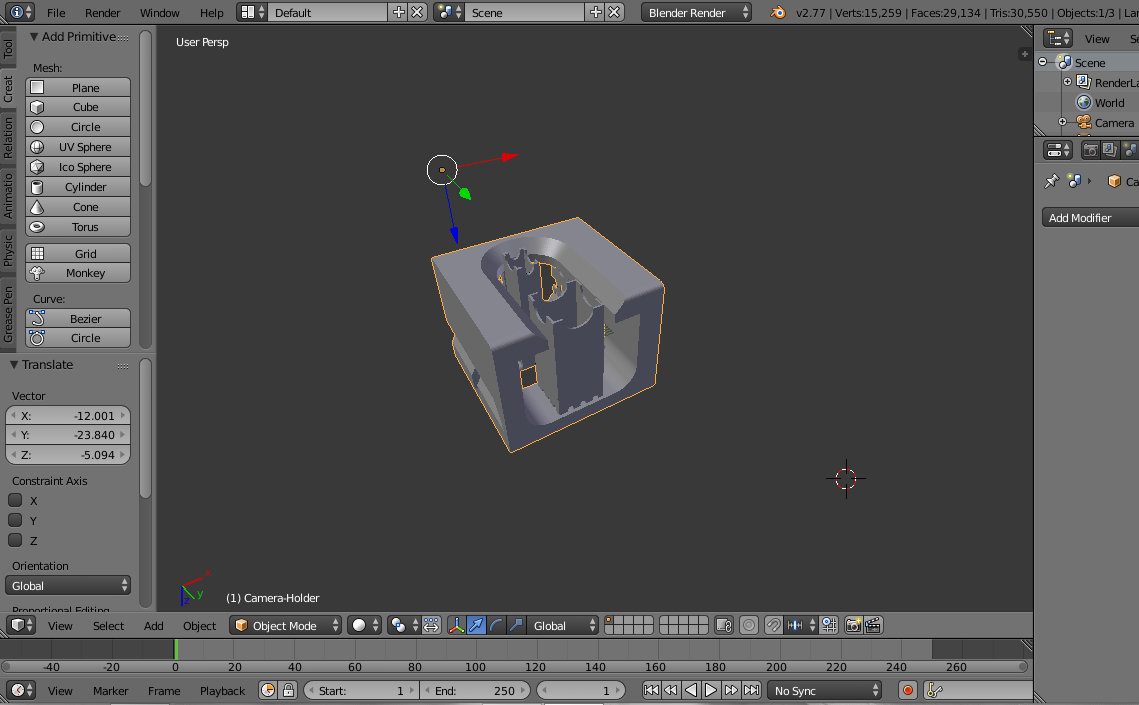
\includegraphics[width=.80\textwidth]{images/cameraBlender.png}}
	}
	\caption{ Diseño 3D de la pinza de agarre en Blender}
\end{figure}

Una vez diseñadas las piezas se ha utilizado Cura, un programa que genera archivos \texttt{.gcode} a partir de diseños 3D. Este tipo de archivos son los que se le envían a la impresora 3D.

\begin{figure}[h]
	\centerline{
		\mbox{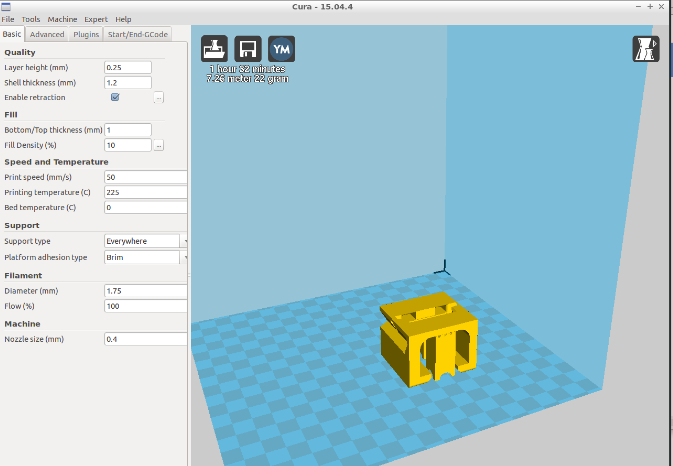
\includegraphics[width=.75\textwidth]{images/Cura2.png}}
	}
	\caption{Imagen de la configuración del Cura para enviar la Pieza de agarre a la impresora 3D}
\end{figure}
 
\newpage
\subsection{Streaming}
\subsubsection{Raspberry Pi3}
El primer elemento en el streaming de video es la Raspberry Pi, que tiene conectada por usb una cámara.

Para recoger el video y mandarlo en tiempo real utilizamos la librería mjpeg-streamer, disponible en github.

Mjpeg-streamer es una aplicación en linea de comandos que permite crear un servidor, para retransmitir imágenes JPG sobre una red basada en IP, desde la cámara hasta un navegador convencional.

Soporta la compresión por hardware (GPU, Unidad de Procesamiento Gráfico) de la cámara, en nuestro caso H.264 Advanced Video Coding (AVC) Standard, que es el compreso de la Webcam Logitech.

Esto permite reducir drásticamente el uso de la CPU de este servidor, haciendo está aplicación un servicio ligero.

El puerto que emplea es el 8080

\begin{figure}[h!]
	\centerline{
		\mbox{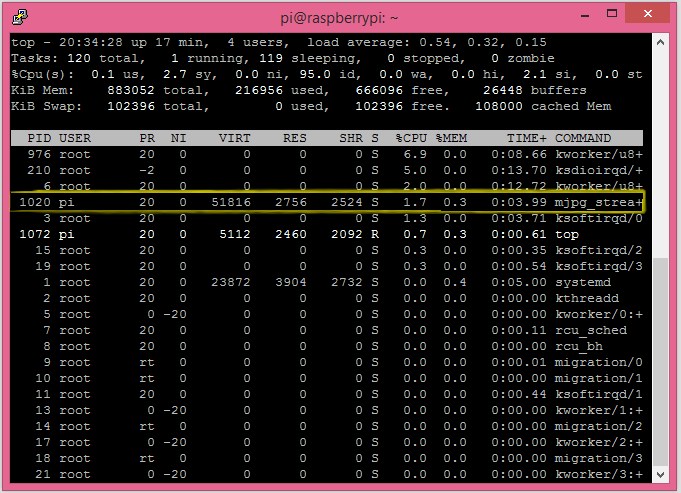
\includegraphics[width=.80\textwidth]{images/UsoCPUMjpeg.png}}
	}
	\caption{Uso de CPU del programa Mjpeg-Streamer por el que se hae el streaming de video}
\end{figure}


Para iniciar el streaming debemos ejecutar un script \texttt{Streaming} que manda el siguiente comando: \texttt{./mjpg\_streamer -i "./input\_uvc.so -d /dev/video0" -o "./output\_http.so -w ./www"}.



\begin{figure}[h!]
	\centerline{
		\mbox{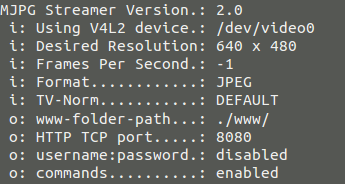
\includegraphics[width=.80\textwidth]{images/Streamingcomando.png}}
	}
	\caption{Ejecución del comando para iniciar el streaming}
\end{figure}

En este momento la Raspberry empezará a coger el video de la cámara y transmitirlo en tiempo real a la siguiente url: \texttt{http://192.168.1.33:8080/stream.html}

\begin{figure}[h!]
	\centerline{
		\mbox{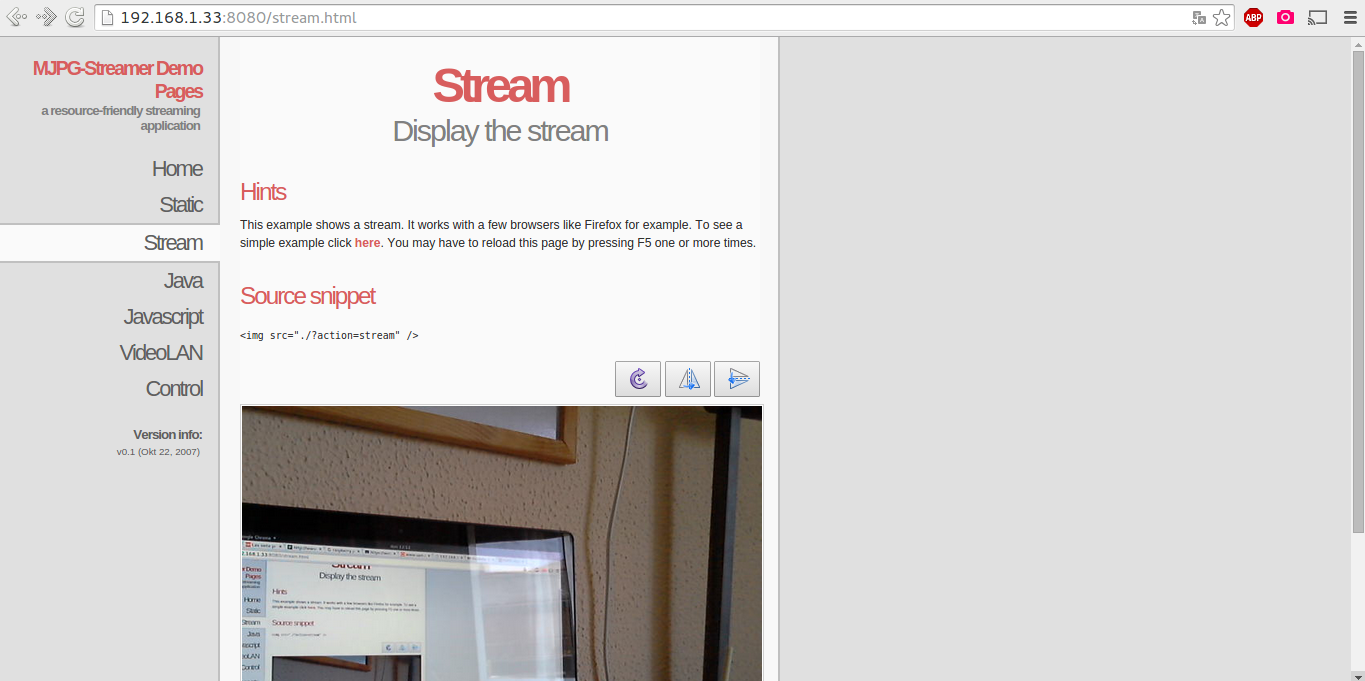
\includegraphics[width=.80\textwidth]{images/pagStream.png}}
	}
	\caption{Página html donde se recibe el streaming a tiempo real desde la Raspberry }
\end{figure}



\newpage
\subsubsection{Ordenador}
El ordenador accede a la IP donde mjpeg-streamer está retransmitiendo el video y lo recoge a través del reproductor de video VLC.

Para ello especificamos en VLC que el medio de reproducción será una ubicación de red.

Posteriormente dividimos el video en dos pantallas exactamente iguales para poder verlo desde las Oculus en modo SBS (Side by Side).

\begin{figure}[h]
	\centering
	\subfigure[Medio de reproducción-Ubicación de red]{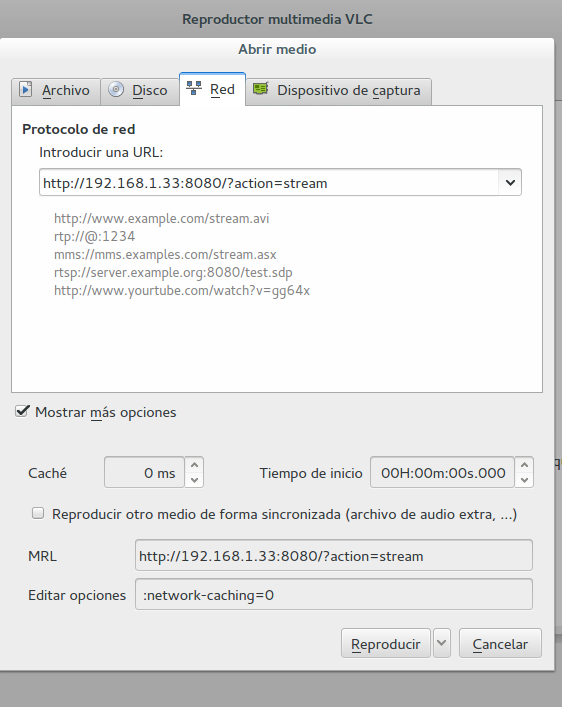
\includegraphics[width=60mm]{images/confVLC.png}}
	\subfigure[División de imágenes]{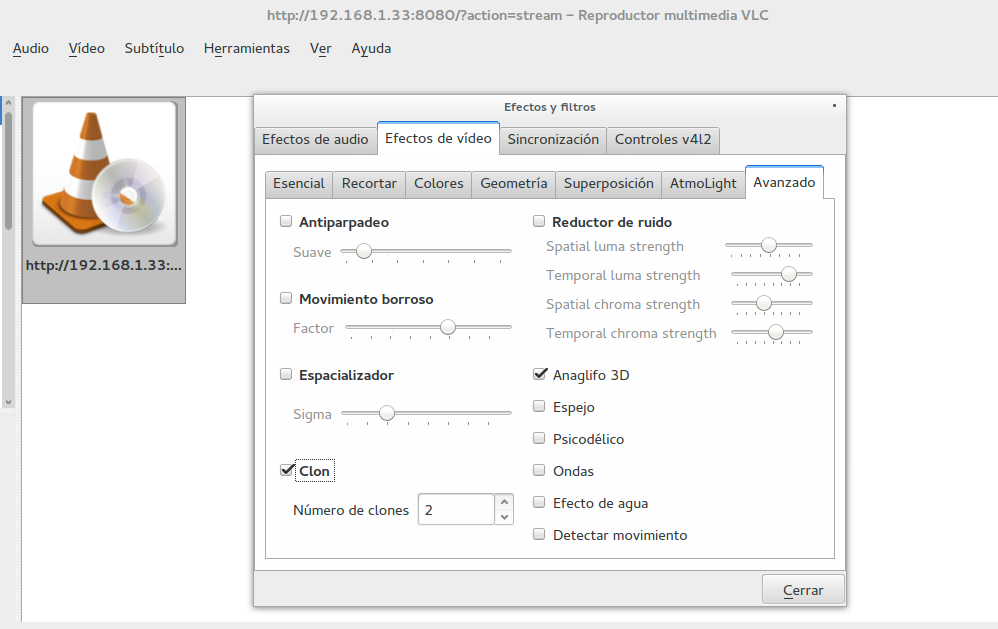
\includegraphics[width=60mm]{images/confSBS.png}}\\
	\subfigure[Reproducción SBS]{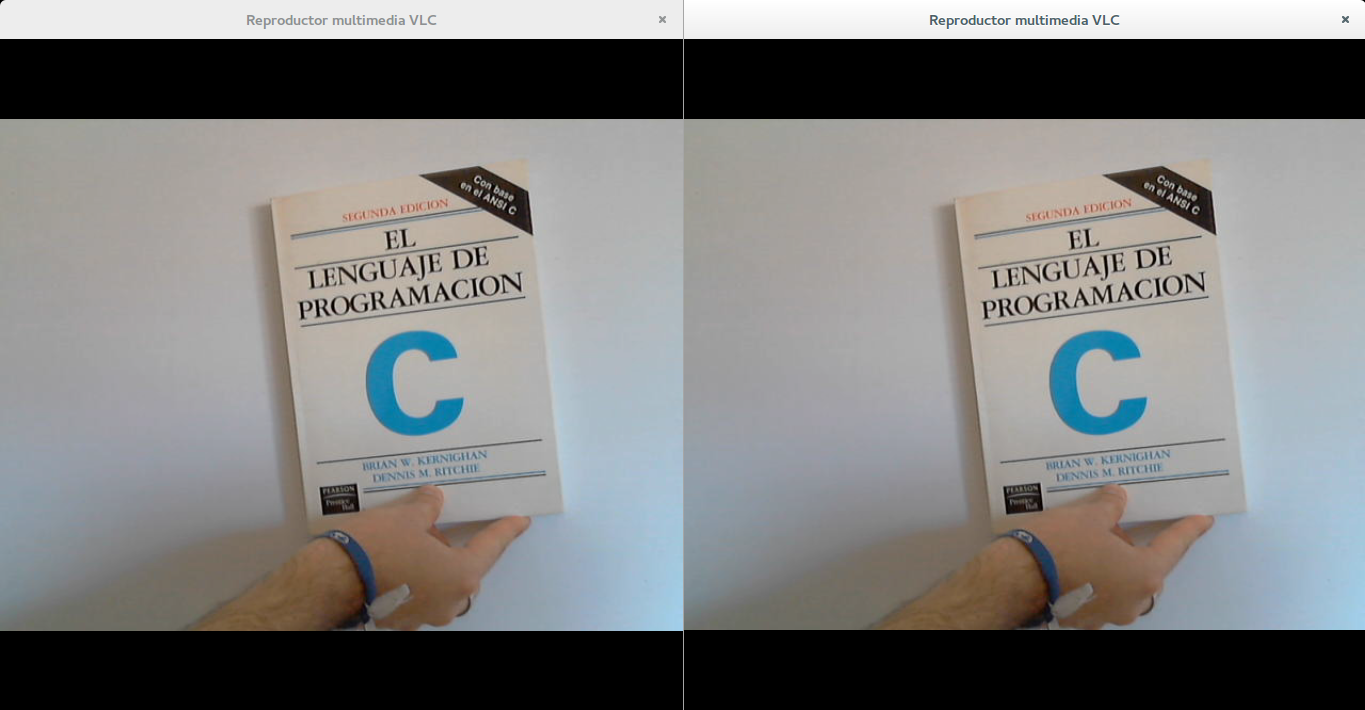
\includegraphics[width=120mm]{images/sbsVLC2.png}} %
		\caption{Configuración y resultado de la reproducción de video en VLC} \label{figstream}
\end{figure}

El ordenador tiene instalado un programa, Virtual Desktop.

Virtual Desktop es una aplicación desarrollada por Oculus Rift y  HTC Vive para utilizar las Oculus Rift en Windows.

Permite ver el escritorio desde las Oculus, pudiendo configurar efectos como ver las imagénes SBS o cambiar el entorno en el que te encuentras (el espacio, una sala de cine...)


%\begin{figure}[h]
%	\centerline{
%		\mbox{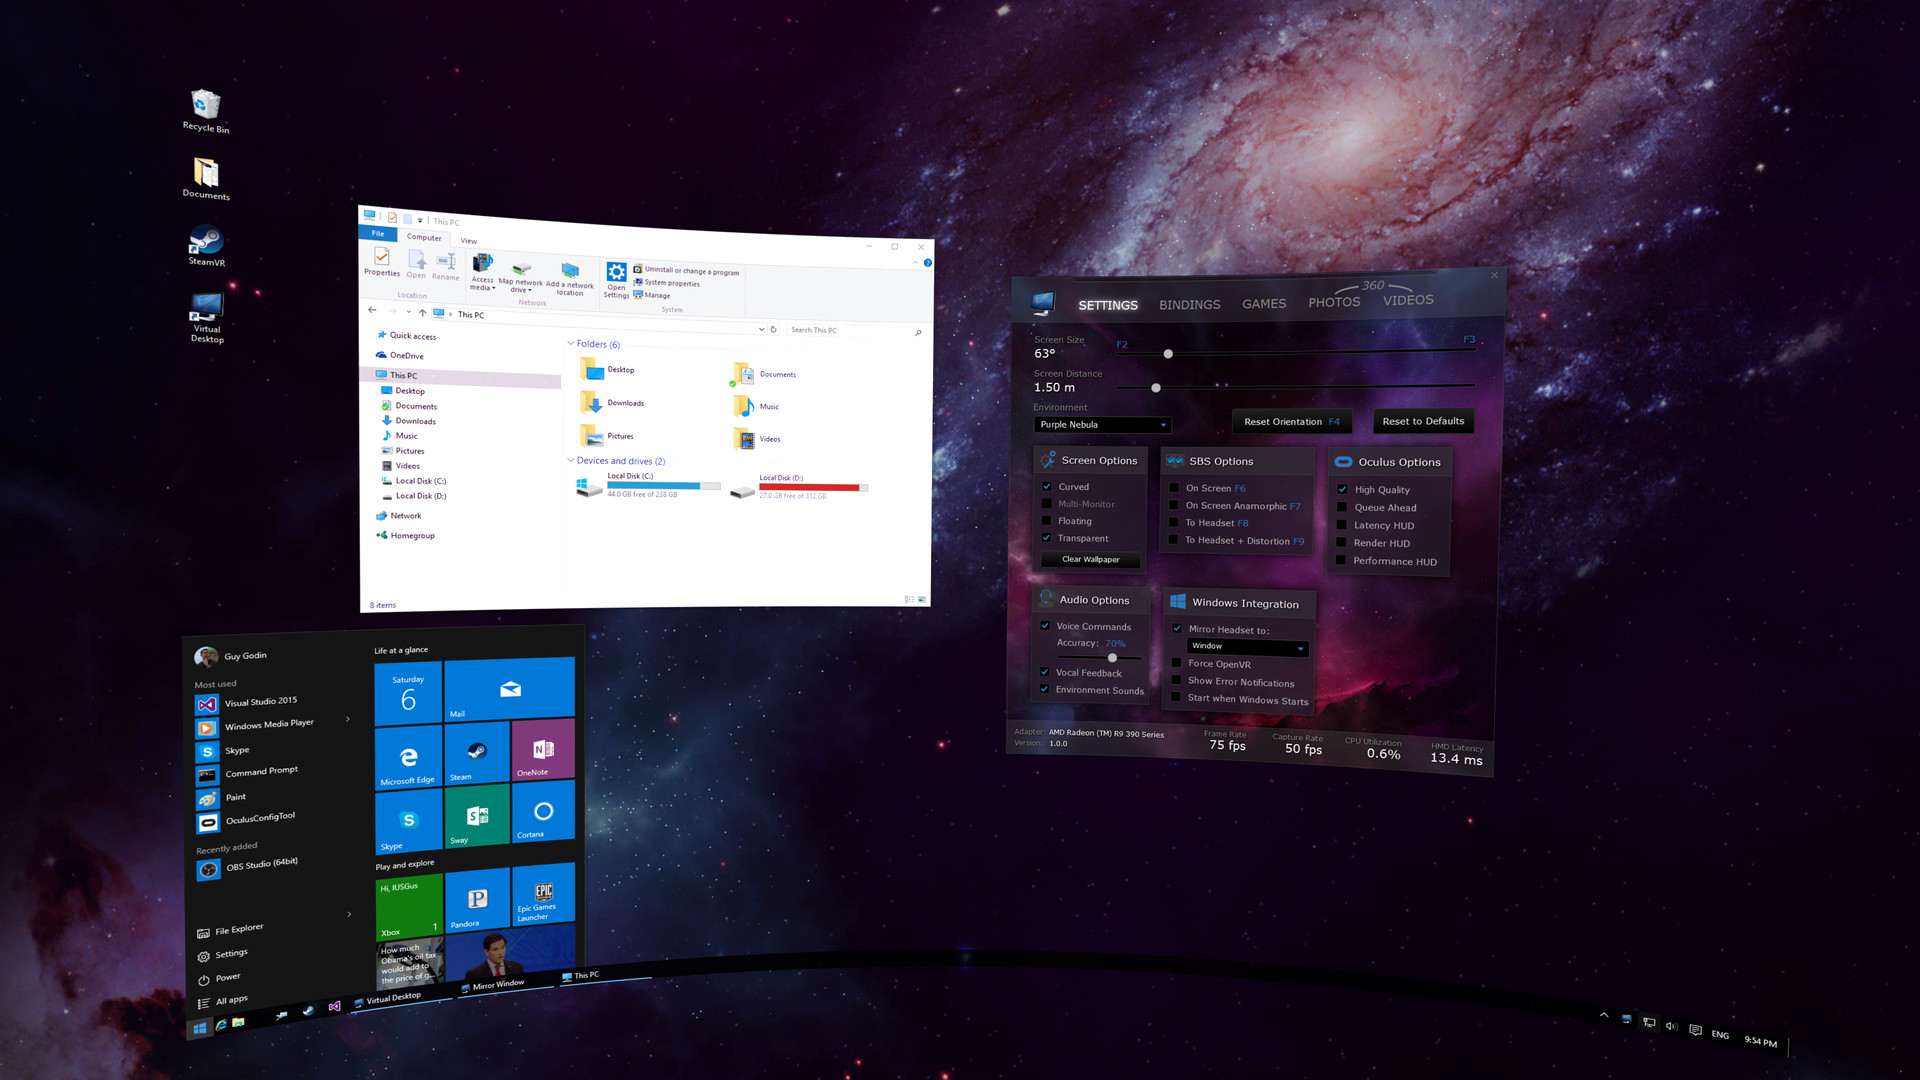
\includegraphics[width=3.00in]{images/VirtualDesktop.jpg}}
%	}
%	\caption{Virtual Desktop}
%\end{figure}

También te permite ver videos descargados en el ordenador y reproducir videos 360.

Nosotros utilizamos la funcionalidad de ver la pantalla del ordenador desde las Oculus con SBS, para visualizar el video que se está reproduciendo en VLC a tiempo real.



\newpage

\subsection{Control del Robot}
El control del robot es el control del movimiento de los tres servos que lo componen. 

Este movimiento se basará en el movimiento de las Oculus, que llevará puestas el usuario.

Por lo tanto el control del robot se divide en tres acciones:
\begin{itemize}
	\item Recogida y procesamiento de la información que mandan las Oculus al ordenador $\rightarrow$ Esto se hará mediante la utilización de la librería \texttt{ovr}.
	
	\item Envío de la información procesada a la Raspberry Pi 3 $\rightarrow$ Para ello el ordenador abrirá dos sockets a través de los cuales mandará los datos al robot
	
	\item Movimiento de los servo motores
\end{itemize}
\paragraph{Recogida y procesamiento de la información que mandan las Oculus al ordenador}


\subparagraph{Librería OVR}
Para recoger desde el ordenador la información que mandan las Oculus utilizamos la librería de Oculus (ovr), escrita en phyton.

La función \textit{ovr.getTrackingState} nos devuelve una estructura (\textit{TrackingState}), que contiene el campo:

\textbf{Pose Statef} HeadPose 
\begin{itemize}
	\item \textbf{Posef} ThePose $\begin{cases}
	\textbf{Quatf} \text{ Orientation}\\
	\textbf{Vector3f}\text{ Position} 
	\end{cases}$
	
	
\end{itemize}

Para obtener la orientación de la cabeza se lee el valor de \textit{HeadPose.ThePose.Orientation.x/y} lo procesa para obtener los grados de orientación de la cabeza y se lo manda a la raspberry a través de sockets.

La información obtenida sobre la orientación respecto al eje $y$ servirá para mover los servos que hay en las ruedas del robot, mientras que la información de $x$ servirá para mover la cámara.


El ordenador crea un servidor y abre dos sockets distintos, uno para la información de $x$ y otro para la de $y$.


De esta forma manejamos los dos movimientos de forma independiente.


\subparagraph{Procesamiento de HeadPose.ThePose.Orientation}

Como se ha dicho en el apartado anterior, la información proveniente de las Oculus nos llega a través de la estructura \texttt{HeadPose}, donde podemos leer el campo \texttt{Orientation} que nos manda la orientación actual de las Oculus Rift en forma de cuaternión.

Para averiguar en qué dirección apuntan las Oculus respecto al eje X guardamos los datos relativos a la posición y la velocidad angular.

 Estos datos son procesados y se le aplican unos parámetros que se han obtenido mediante la realización de pruebas para obtener una correcta calibración.

De este modo se ha podido realizar una conversión de los datos obtenidos por las Oculus a unidades de grados que nos facilitan el control posterior de la posición de los servomotores.

\begin{figure}[h!]
	\centerline{
		\mbox{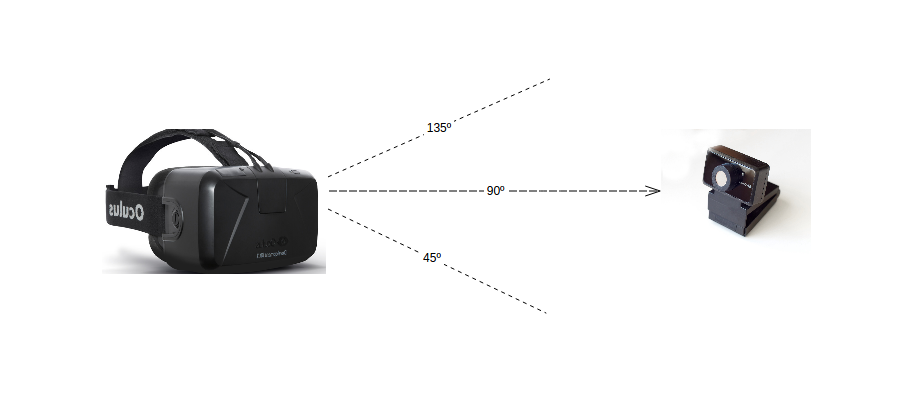
\includegraphics[width=.80\textwidth]{images/Oculusgrados2.png}}
	}
	\caption{Posición de as Oculus respecto al eje X una vez procesados los datos de \texttt{HeadPose.ThePose.Orientation}}
\end{figure}
\newpage
\paragraph{Envío de la información procesada a la Raspberry Pi 3}



Para el control del movimiento del robot es necesario que el ordenador le mande los datos referentes a la posición de las Oculus de forma automática, inmediatamente después de procesarlos.

Con este fin, desde el mismo programa donde se recibe y procesan los datos de las Oculus, el ordenador abre dos sockets, y se queda a la espera de que el robot se conecte.

Recordemos que el ordenador y la Raspberry Pi 3 están dentro de la misma red local (WifiRaspi3), y que ambos tenían IP fija.

La apertura de sockets por parte del ordenador se hace de la siguiente forma:

\lstset{language=python, breaklines=true, basicstyle=\footnotesize}
\begin{lstlisting}[frame=single]

	host = "192.168.1.35"    #IP asignada al ordenador
	port = 4446       #movimiento de la camara
	port2 = 4447      #movimiento de las ruedas

	s = socket(AF_INET, SOCK_STREAM)
	s2 = socket(AF_INET, SOCK_STREAM)

	s.bind((host,port))
	s2.bind((host,port2))

	s.listen(5)
	s2.listen(5)

	q,addr = s.accept()
	q2,addr2 = s2.accept()

\end{lstlisting}

De esta forma, cada vez que se recibe y procesan datos referentes a la posición de las Oculus, se dividen en información para la cáma e información para las ruedas y se ejecutna las instrucciones \texttt{ q2.send(data)}  y \texttt{ q.send(data)} para mandar los datos.
\subparagraph{Recepción de los datos en el robot}

La Raspberry tiene dos programas (uno para las ruedas y otro para la
cámara) que están escuchando continuamente lo que manda el ordenador y en
cuanto recibe el comando lo manda a los servos.

Para ello, al iniciarse cada programa, se conectan al socket correspondiente
\lstset{language=python, breaklines=true, basicstyle=\footnotesize}
\begin{lstlisting}[frame=single]
	host = "192.168.1.35"
	port=4447
	s=socket(AF_INET, SOCK_STREAM)
	s.connect((host,port))
\end{lstlisting}

Y se ponen a escuchar (\texttt{msg=s.recv(1024)})hasta que les llegan los datos.

Una vez que tiene los datos los transforma en comandos válidos para los servomotores,tal y como se explia en el siguiente apartado, les manda la instrucción y vuelve a escuchar.


\paragraph{Movimiento de los servo motores}



Como ya se indicó en la sección (seccion de los servos,PWM, etc..) el movimiento de los servos se controla con una señal PWM (Pulse With Modulation).

Por ello utilizamos la librería RPi.GPIO, que ofrece funciones para PWM.

Hay dos parámetros principales para determinar el pulso que se envía al motor:
\begin{itemize}
	\item \textbf{Frecuencia} : veces por segundo que se genera el pulso.
	\item \textbf{Duty cycle} : es el porcentaje de tiempo que el pulso está arriba. (recordemos que la señal es una señal cuadrada)
\end{itemize}


Veamos un ejemplo para clarificar esto:

\subparagraph{PWM- Frecuencia:50Hz , DutyCycle $50\%$}



Si fijamos una frecuencia de 50Hz estaremos mandando una señal de 50 pulsos por segundo, es decir, un pulso cada $0.02$ segundos.

Al poner un DutyCycle al $50\%$ estamos estableciendo que durante esos $0.02$ segundos el pulso estará $0.01$ segundos en posición "High" y el resto del tiempo en posición "Low".


\subparagraph {PWM- Frecuencia:50Hz , DutyCycle $80\%$}

Si fijamos una frecuencia de 50Hz, como la del ejercicio anterior pero por el contrario ponemos un DutyCycle del $80\%$ tendremos:
\begin{itemize}
	\item 1 pulso cada $0.02$ segundos
	\item El pulso estará en posición "high" el $80\%$ del tiempo ($0.016$ segundos) y en posición "low" los otros $0.004$ segundos restantes.
\end{itemize}



La Raspberry Pi recibe a través de los sockets el ángulo de orientación de la cabeza sobre el eje y o x.


Esta información se procesa de forma distinta según si queremos mover el servo de la cámara o las ruedas del robot.

Esto es porque los servos de las ruedas son de rotación continua, a diferencia que el de la cámara.

\subsubsection{Control de los motores de las ruedas del robot}

Los motores que mueven las ruedas del robot son dos servo motores que están modificados para tener rotación continua. El funcionamiento de los servo motores de rotación continua ya se ha explicado en la sección de análisis.

Recordamos muy brevemente que en los servo motores de rotación continua, la pulsación que le mandas al motor no indica la posición en la que debe colocarse si no la velocidad a la que debe rotar.

Para controlar nuestro robot se ha fijado una velocidad constante de giro en base a pruebas experimentales de la velocidad de movimiento de cabeza medio en una persona.

Por lo tanto , si queremos rotar nuestro robot hasta una posición concreta la variable no es la velocidad si no el tiempo durante el que rotan los motores.

Para calcular dicho tiempo se midió experimentalmente cuanto tardaba el robot en girar 90º. El resultado fueron 0.5 segundos por lo que 
$$90 / 0.5 = 0,005555556 \text{ segundos en girar un grado}$$

De esta forma, cuando el robot recibe una posición en grados desde el ordenador ejecuta las siguientes instrucciones:


$\begin{cases}
\text{Grados recibidos del ordenador = g}\\
dif = |posActual-g|\rightarrow\text{ Se calcula el número de grados que tiene que moverse}\\
\text{Rotar motores derecho e izquerdo}\\
time.sleep((dif*0.005555) \rightarrow \text{ Rotamos el tiempo necesario alcanzar la posición}\\
\text{Parar motores derecho e izquerdo}
\end{cases}$



\subsubsection{Control del motor de la cámara del robot}

La cámara se mueve gracias a un servo motor cuyo rango de movimiento va de 0 a 180 grados.

Este motor se mueve por pulsos, tal y como se explica en la sección de Análisis.

La Raspberry recibe un ángulo que indica hacia donde están orientadas las Oculus en ese momento.

Para transformar este ángulo el pulso(PWM) correspondiente debemos tener en cuenta que un servo requiere una señal PWM con un periodo de 20 ms y un ancho de pulso entre $0.9$ y $2.1$ ms.

Ya que el servo tiene un rango de ángulos de 0 a 180 grados, es fácil ver que el ancho de pulso de $0.9$ ms se corresponde con 0º y $2.1$ ms con 180º

Asi podemos convertir los ángulos en pulsos PWM y mover la cámara hacia la dirección deseada.

\paragraph{Control del Robot por parte del usuario}

El las anteriores secciones se ha explicado el funcionamiento interno del control de movimientos del robot.

En este nuevo apartado se presenta cómo debe utilizar el usuario este producto, qué rango dde movimiento tiene y cómo puede hacer avanzar el robot.

\subsubsection{Instrucciones de mando}

Como se especifica al inicio de este trabajo, el robot estará controlado exclusivamente por el movimiento de cabeza del usuario.

Para ello se debía idear una forma cómoda e intuitiva de mandar instrucciones al robot.

Diferenciamos dos estados de movimiento del robot:
\begin{itemize}
	\item Exploración$\rightarrow$ En este estado el robot no avanza, solo explora lo que tiene a su alrededor. Esto lo hace moviendo la cámara o rotando sobre sí mismo.
	\item Transporte $\rightarrow$ El robot avanza hacia delante.
\end{itemize}

Finalmente se ha implementado de la siguiente forma:


\begin{figure}[h]
	\centering
	\subfigure[Rotación sobre sí mismo]{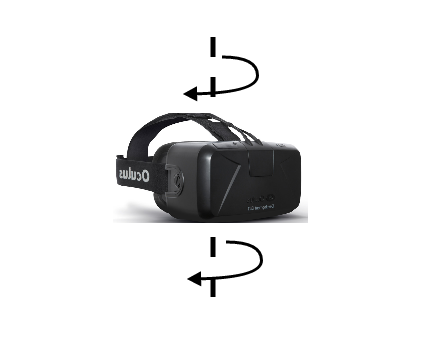
\includegraphics[width=60mm]{images/Robotrota.png}}
	\subfigure[La cámara gira respecto del eje X]{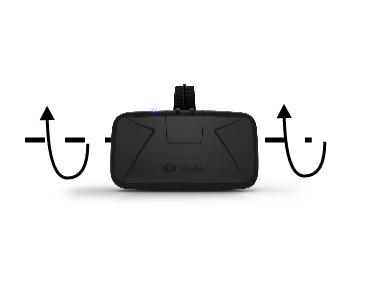
\includegraphics[width=60mm]{images/Robotexp.png}}\\
	\subfigure[Movimiento hacia delante si el ususario baja la cabeza]{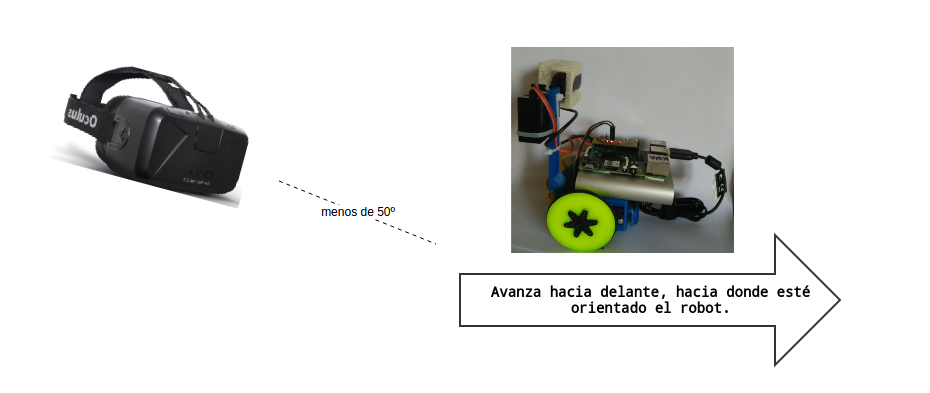
\includegraphics[width=120mm]{images/RobotAv.png}} %
	\caption{Posibles movimientos del robot según el movimiento de las Oculus Rift} \label{movRobot}
\end{figure}

Como viene explicado en la imagen, si el usuario mira hacia los lados el robot rotará sobre sí mismo sin moverse del sitio, hacia la dirección que señalen las Oculus Rift.

Si el usuario mueve la cabeza hacia arriba o hacia abajo sin llegar a menos de 50º, la cámara se moverá como si fuera la cabeza del usuario.

En el caso de que el usuario oriente la cabeza hacia abajo, con un ángulo menor de 50º respecto al eje Y, la cámara se orientará horizontalmente (90º respecto al eje Y) y el robot avanzará hasta que el usuario cambie la posición de la cabeza

\chapter{Pruebas y Resultados}

A continuación se explican las pruebas y los resultados obtenidos tras desarrollar el proyecto.

\section{Latencia de recepción de comandos}

Para probar el sistema primero hemos hecho pruebas del funcionamiento de la red local, ya que en este trabajo es esencial tener poca latencia.

Para ello se ha probado el alcance de la red inalámbrica, mandando comandos a los servo motores desde el ordeador.

A continuación se ven los resultados obtenidos tras mandar comandos a una distancia de 7,5 metros y mandar comando estando el robot y el ordenador en habitaciones separadas

\begin{figure}[h!]
	\centerline{
		\mbox{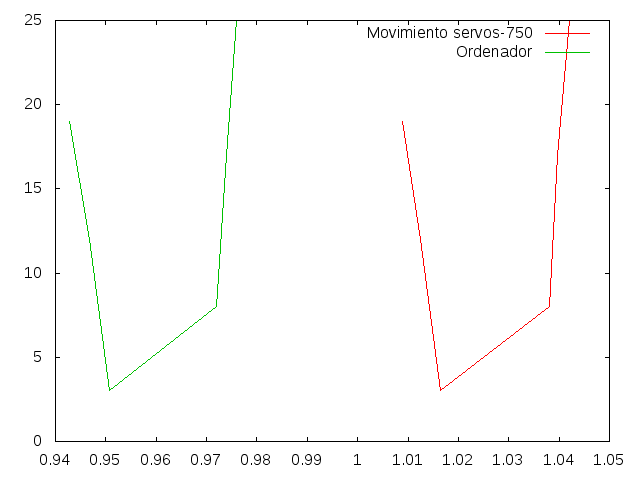
\includegraphics[width=.80\textwidth]{images/Temp_750.png}}
	}
	\caption{Diferencia de tiempos entre envío y recepción de comandos a 7,50 metros}
\end{figure}

\begin{figure}[h!]
	\centerline{
		\mbox{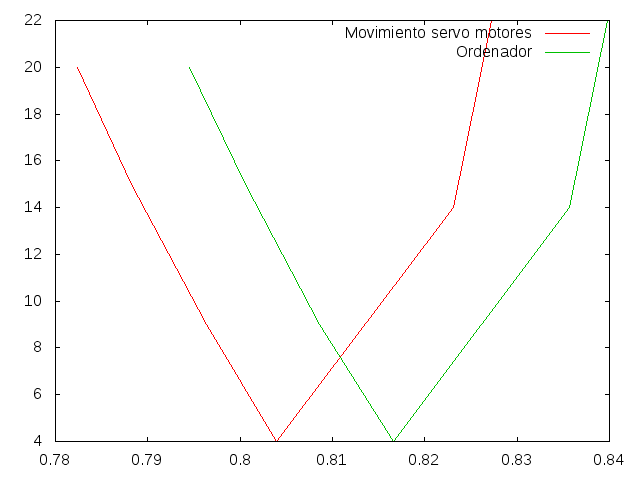
\includegraphics[width=.80\textwidth]{images/Temp_fuera.png}}
	}
	\caption{Diferencia de tiempos entre envío y recepción de comandos a 7,50 metros}
\end{figure}

Vemos que la latencia entre la medición en las Oculus y la recepción en la Raspberry es muy pequeña.

En la gráfica que nos muestra la diferencia de tiempos a 7,5 metros vemos que de media el comando tarda en transmitirse menos de 0.5 segundos.

En las pruebas entre habitaciones separadas, vemos que la diferencia no pasa de los 0,5 segundos por lo que creemos que es una latencia asumible ya que el robot no va a grandes velocidades.
\newpage

\section{Feedback de los usuarios}

Se han hecho pruebas de control a usuarios para comprobar su usabilidad.

Las primeras pruebas han sido de calibración. Un usuario ha aprendido a controlar el robot y ha pedido cambios para que el manejo sea más intuitivos.

Tras hacer los cambios pedidos por el primer usuario se ha pedido a distintas ersonas que hagan diversas acciones con el robot y que puntúen la facilidad de realizar dichas acciones.

\paragraph{Cambios realizados en la fase de calibración}
\begin{itemize}
	\item \textbf{Se ha reducido la velocidad de giro de los motores de las ruedas}.
	
	\item \textbf{Se ha modificado la forma de girar}. En las primeras pruebas el robot giraba de forma que siempre apuntaba al mismo sitio que la cabeza del usuario.
	
	Esto era bastante incómodo porque para dar la vuelta el usuario debia girar sobre sí mismo.
	
	Además para avanzar hacia la derecha o hacia la izquierda el usuario debía estar mirando en esa dirección.
	
	Esto se ha modificado de forma que si la cabeza del usuario está orientada en un ángulo mayor de 110 grados (siendo 90º la posición frontal natural) el robot girará continuamente hacia la derecha hasta que el usuario vuelva a mirar al centro.
	
	El giro hacia la izquierda se hace de la misma forma.
	
	\item \textbf{Se ha modificado la forma de parar}.Cuando el usuario mira hacia abajo el robot avanza.
	
	En las primeras pruebas el usuario debía girar hacia la derecha o hacia la izquierda para dejar de vanazar.
	
	Esto se ha modificado de forma que ahora para parar el usuario deberá colocar la cabeza en la posición central natural (90º respecto al eje Y)
\end{itemize}

\paragraph{Valoración de los usuarios}

Se ha pedido a los usuarios que realicen las siguientes acciones:

\begin{itemize}
	\item Girar a la derecha
	\item Girar a la izquierda
	\item Mirar hacia arriba
	\item Estar 30 segundos aproximadamente girando el robot sobre sí mismo hasta tener controlado el giro.
	\item Andar hacia delante
	\item Parar
	\item Estar cerca de un minuto paseando para familiarizarse con los movimientos.
	\item Fijar un objetivo y alcanzarlo.
\end{itemize}

La siguiente tabla muestra la valoración de los usuarios tras realizar las pruebas.

\begin{tabular}{|l | c | c | c | c | c | r | r |}
	\hline
	 & U1 & U2 & U3 & U4 & U5 & U6 & U7\\
	\hline
	Giro derecha & 9 & 6 & 6 & 4 & 5 & 5 & 6\\
	Giro izquierda & 7.5 & 4 & 6 & 4 & 5 & 5 & 7\\
	Mirar hacia arriba & 9 & 10 & 9 & 10 & 9 & 9 & 9\\
	Andar & 10 & 8 & 10 & 8 & 8 & 9 & 9\\
	Parar & 9 & 10 & 9 & 7 & 7 & 7 & 8\\
	Alcanzar un objetivo & 8.5 & 6 & 8 & 7 & 5 & 5 & 8\\
	Sensación de Control & 7.5 & 6 & 9 & 4 & 5 & 4 & 7\\
	Facilidad de aprendizaje & 9 & 8 & 10 & 10 & 9 & 8 & 10\\
	\hline
\end{tabular}


\paragraph{Comentarios tras las pruebas}


Los comentarios más usuales tras utilizar el robot han sido:
\begin{itemize}
	\item El robot gira demasiado deprisa.
	\item Sería bueno incluir un micrófono en el robot ya que marea un poco el mirar un espacio desde el robot y estar oyendo los ruidos del espacio en el que realmente estoy.
	\item Es muy intuitivo la forma de controlar el robot.
	\item Cuanto más lo uso más fácil me es controlarlo.
\end{itemize}
 
Las coclusiones tras analizar los resultados se exonen en e siguiente capítulo.

\chapter{Conclusiones y trabajo futuro}
\label{chap:conclusiones}
\vspace{-0.2cm}

\section{Conclusiones}
En este apartado analizaremos los resultados obtenidos, hablaremos de posibles mejores y se expondrán las conclusiones del proyecto.

\paragraph{Puntos positivos y a mejorar}

Tras las pruebas se ve que el mayor defecto del proyecto es la \textbf{velocidad de giro} de los motores de las ruedas.

La calibración de servo motores es una tarea que se resuelve de forma experimental. La dificultad que nos encontramos es que la velocidad de giro cambia según en la superficie en la que se encuentre el robot por lo que habría que realizar las pruebas en diferentes entornos y hacer una calibración media.

Los usuarios han estado cada uno menos de 7 minutos con el robot y \textbf{todos menos uno lograron alcanzar su objetivo} en menos de un minuto, por lo que es una \textbf{aplicación fácil de manejar y de aprender}, como se ha visto en las valoraciones.

Otro problema es el \textbf{alcance de red de la Raspberry Pi 3}. Si el robot se alejaba mucho del router los servos seguín recibiendo correctamente los comandos pero el streaming tenía algo más de latencia.

Además la \textbf{Raspberry Pi 3 necesita de más amperaje que la Raspberry Pi 2} por lo que se concluye que por ahora, y hasta que se mejore la Raspberry Pi 3, es mejor utilizar Raspberry Pi 2 con un pincho Wifi para poder conectarse a la red local.

De esta forma se consigue mayor alcance de red y se necesita menos Amperios para alientar la placa.

A pesar de todos estos puntos a mejorar el resultado es muy bueno, teniendo e cuenta que e una primera aproximación a lo que que pretende ser un proyecto futuro.

Además es un proyecto con una \textbf{muy buena acogida}, a todos los usuarios les ha resultado ameno hacer las pruebas y ver cómo iban mejorando.

También es fácil de desarrollar con las herramientas de las que disponemos y con \textbf{mucho potencial}, ya que incluye dos tecnologías que están en pleno desarrollo y que aún tienen mucho que avanzar.

Otra ventaja es que hace uso de dispositivos de \textbf{fácil acceso} por lo que no resultaría demasiado caro de fabricar.

\subsection{Tecnologías aprendidas}

Durante la realización de este proyecto he utilizado muchas tecnologías, alguna de ellas completamente nuevas para mi.

El ejemplo más claro de esto son las gafas de realidad virtual Oculus Rift. Ha sido una suerte tener acceso a ellas y poder aprender a utilizar algunas de las librerías que hay disponibles para los desarrolladores.

También ha sido una sorpresa descubrir la gran variedad de posibilidades a desarrollar que permiten las Oculus, como es este proyecto.

He afianzado los conocimientos de robótica que ya tenía. Todo lo que sabía de robótica lo había aprendido en el Club de Robótica de esta universidad y gracias a este trabajo he podido aplicarlos y aumentarlos.

Todo el proyecto está desarrollado en python, lenguaje de programación que no he utilizado en ninguna asignatura de la carrera y que solo había visto muy por encima para proyectos sencillos.
Durante este proyecto he aprendido a utilizar las librerías de python disponibles para las Oculus Rift y para el control de servomotores.

La placa base del robot es una Raspberry Pi 3, que tampoco había tenido la oportunidad de utilizarla nunca. De todas formas esto no ha sido novedoso para mi porque sí había participado en algún proyecto sencillo con Raspberry.

En conclusión este trabajo ha sido muy instructivo y ha ampliado de forma significativa mis conocimientos sobre robótica y realidad virtual.



\section{Trabajo futuro}
Este trabajo es solo el inicio de lo que podría ser un proyecto muy interesante.

El robot que hemos construido es una extensión del sentido de la vista, pero se podría construir un robot controlado por una persona y que fuera la extensión de todos sus sentidos,permitiendo así conocer y sentir el mundo sin necesidad de moverse de su casa.

Además la realidad virtual es una herramienta muy potente, que no solo te permite modificar tu mundo a placer sino que te premita crear entornos totalmente distintos. Se podría estudiar cómo interactuar con ese mundo virtual no solo a través de la vista , sino con todos los sentidos.

Otro camino por el que se puede investigar es la unión de este proyecto con la domótica.
Creo que en un futuro no muy lejano, las casas serán casas domotizadas, que igual que se podrán controlar desde el móvil podremos controlass con las gafas de realidad virtual.

\backmatter
\appendix

\cleardoublepage

\nocite{*}
\bibliography{hpcap40g}{}

\cleardoublepage
\printindex

\end{document}
